% Fix: From https://tex.stackexchange.com/a/508995/108670
\RequirePackage{snapshot}
\makeatletter
\def\snap@providesfile#1[#2]{%
  \wlog{File: #1 #2}%
  \if\expandafter\snap@graphic@test\expanded{#2}@@\@nil
    \snap@record@graphic#1\relax #2 (type ??)\@nil
  \else
    \expandafter\xdef\csname ver@#1\endcsname{#2}%
  \fi
  \endgroup
}
\makeatother

\documentclass[twoside,a4paper,11pt]{memoir}
\usepackage{document}
\usepackage[outputdir=../out]{minted}
\usepackage{todonotes}
\usepackage{bussproofs}
\usepackage{subcaption}
\usepackage{amsfonts}
\usepackage{formal-grammar}
\usepackage{lineno}
\usepackage{soul}
\usepackage{mdframed}
% \usepackage{syntax}

% Grammar references in cref
\crefname{floatgrammar}{Grammar}{Grammars}

% textbt = bold texttt
\newcommand{\textbt}[1]{\textbf{\texttt{#1}}}

\newcommand{\prodname}[1]{{\scriptstyle <}\textit{#1}{\scriptstyle >}}

% Prevent footnotes from splitting across pages.
\interfootnotelinepenalty=100000

% Add \@ _before_ the terminating period of the sentence (`UI\@. Test`)
% to allow inter-sentence spacing when the sentence ends with a capital letter.

\newminted[dynamix]{spoofax_lexer.py -O "parseTable=spoofax/dynamix/sdf.tbl,esv=spoofax/dynamix/editor.esv.af" -x}{linenos,frame=single,framesep=2pt}
\newminted[sdf3]{spoofax_lexer.py -O "parseTable=spoofax/sdf3/sdf.tbl,esv=spoofax/sdf3/editor.esv.af" -x}{linenos,frame=single,framesep=2pt}
\newminted[statix]{spoofax_lexer.py -O "parseTable=spoofax/statix/sdf.tbl,esv=spoofax/statix/editor.esv.af" -x}{linenos,frame=single,framesep=2pt}
\newminted[stratego]{spoofax_lexer.py -O "parseTable=spoofax/stratego/sdf.tbl,esv=spoofax/stratego/editor.esv.af" -x}{linenos,frame=single,framesep=2pt}
\newminted[tim]{spoofax_lexer.py -O "parseTable=spoofax/tim/sdf.tbl,esv=spoofax/tim/editor.esv.af" -x}{linenos,frame=single,framesep=2pt}
\newminted[mat]{spoofax_lexer.py -O "parseTable=spoofax/mat/sdf.tbl,esv=spoofax/mat/editor.esv.af" -x}{linenos,frame=single,framesep=2pt}
\newminted[dynsem]{spoofax_lexer.py -O "parseTable=spoofax/dynsem/sdf.tbl,esv=spoofax/dynsem/editor.esv.af" -x}{linenos,frame=single,framesep=2pt}
\newminted[plain]{text}{linenos,frame=single,framesep=2pt}

\addbibresource{document.bib}
\addbibresource{researchr.bib}

% !TEX root = document.tex

\title{Dynamic semantics in Spoofax}
\subtitle{Version of \today}
%\subtitle{Master's Thesis}
\author{Thijs Molendijk}
\authoremail{\url{t.molendijk@student.tudelft.nl}}
\birthplace{Ede, the Netherlands}
\studentid{4730739}
\coverpicture{\includegraphics[width=13cm]{./img/maze.ps}}
\colophon{\noindent
  \copyright{} \the\year{} \: \theauthor. \\[1em]
  Cover picture: Random maze.
}


\begin{document}
% \linenumbers

\frontmatter
\thispagestyle{empty}
\maketitle
\makeformaltitlepages{% !TEX root = document.tex

Abstract here.
\todo{abstract}}

% !TEX root = document.tex

\chapter{\label{ch:Preface}Preface}
\addcontentsline{toc}{subsection}{Preface}
Preface here.
\todo{preface}

\vspace{1cm}
\begin{flushright}
  \theauthor{}\\
  Delft, the Netherlands\\
  \today{}\\
\end{flushright}


\cleardoublepage\tableofcontents
% \cleardoublepage\listoffigures
% \cleardoublepage\listoftables
\cleardoublepage\listoftodos
\cleardoublepage\mainmatter{}

\todo[inline]{Double check figure placement/positions across all chapters}

% !TEX root = ../document.tex

\chapter{\label{ch:introduction}Introduction}

\todo{not entirely sure about this introduction}

While the advent of computing has brought with it a large swathe of programming languages, wildly varying in levels of abstraction, capabilities, and usecases, we can reduce each of them down to just three components acting in unison to form a "programming language": the grammar, the static semantics, and the dynamic semantics.\\

The grammar governs how the programmer writes code. It specifies what lexical structures the language expects, what keywords, operators, literals, expressions it supports, and how the language converts this textual representation to a format more suitable to work on, the \ac{AST}.\\

The static semantics govern what programs have \textit{meaning}. It encompasses all rules that can be checked at compile time, such as the validity of name binding within the program and whether it does not violate any typing rules. Some languages thrive around (strict) static semantics, whereas other languages, particularly dynamic scripting languages, may not have any at all.\\

Finally, the dynamic semantics of a language describe \textit{how} a program runs. It formalizes that an addition of two numbers will indeed lead to a single number that is the sum of the two. At the same time, it describes what might happen to the result should the addition of the numbers overflow.\\

% ---

It is the collection of these properties that forms a programming language, not a specific implementation. Anyone can write a compiler for the \Cplusplus 98 programming language, as long as they adhere to the formal specification of \Cplusplus 98 as written in ISO/IEC 14882:1998 \cite{ISO:1998:IIP}. Someone wanting to implement a new JavaScript engine needs only to follow ECMA-262 \cite{ecma1999262}. Any virtual machine compliant with the Java Language Specification \cite{10.5555/2636997} is able to run any and all valid Java programs.\\

That's the theory, at least. In practice, bugs in implementations, ambiguities in the natural language used in the specification, as well as choices left up to the implementation mean that even trivial \Cplusplus programs that run flawlessly when compiled by GCC \cite{gcc} may behave entirely different when compiled by LLVM's Clang \cite{clang}. Which one of the observed behaviors is the \textit{correct} one can only be judged by consulting the specification.\\

Many other programming languages, even extremely popular ones, do not have a specification. This is completely understandable. After all, it is a herculean task to formally describe every construct and behavior in one's programming language. For these languages, the reference implementation of the language \textit{is} the specification. Creating an alternative implementation of these programming languages amounts to carefully observing and replicating what the reference compiler does, and ensuring that this behavior stays consistent with the reference as both implementations continue to improve and evolve.\\

\todo{needs a better segue into dynamix, something about why dynamix helps solve these issues}

% ---

In this thesis, we introduce a new \ac{DSL} called Dynamix for use in the Spoofax language workbench \cite{Spoofax2021}. Dynamix aims to unify the specification and implementation of the dynamic semantics of a programming language, by offering a language that is high-level enough to function as a formal specification of the language, while at the same time allowing this specification to be turned into an efficient compiler for the language.\\

An example of Dynamix in action can be seen in \cref{fig:dynamix_addition}. It describes that the addition operator should be implemented by evaluating the values of each sub-term in left-to-right order, then yielding the 32-bit signed addition result of the two values. The Dynamix source has exactly the same behavior as the analogous formal definition.\\

\begin{figure}
  \begin{prooftree}
    \AxiomC{$G \vdash l \Downarrow i_1 $}
    \AxiomC{$G \vdash r \Downarrow i_2 $}
    \AxiomC{$v = i_1 +_{\textrm{signed 32-bit}} i_2$}
    \TrinaryInfC{$G \vdash l \textrm{ + } r \Downarrow v$}
  \end{prooftree}
  \begin{dynamix*}{firstline=3,firstnumber=1}
module main

rules
  compileExpr(Add(left, right)) = {
    lv <- compileExpr(left)
    rv <- compileExpr(right)
    #i32-add(lv, rv)
  }
  \end{dynamix*}
  \caption{A formal dynamic specification for the behavior of integer addition (top), and an equivalent Dynamix specification expressing the same behavior (bottom).}
  \label{fig:dynamix_addition}
\end{figure}

Dynamix is designed to be used within the Spoofax language workbench \cite{Spoofax2021}, an environment designed for the design and implementation of (domain-specific) programming languages. Within Spoofax, Dynamix can provide additional static analysis based on the algebraic signature of the source language, interact with the results of static analysis, and be invoked as part of a language implementation test-suite.\\

\noindent This thesis makes the following contributions:

\begin{itemize}
  \item We introduce Tim, a language-agnostic intermediate representation for programs and the output format for Dynamix.
  \item We introduce Dynamix, a programming meta-language used for describing the dynamic specification of a programming language.
  \item We present two \todo{three?} case studies that evaluate the performance and capabilities of Dynamix by implementing Dynamix specifications for the ChocoPy programming language \cite{PhadyeSH19-SPLASHE} extended with exception handling, and a subset of the Stratego \cite{Visser05-SCAM} programming language.
\end{itemize}

\noindent The remainder of this document is structured as follows:

\begin{itemize}
  \item We briefly introduce the Spoofax language workbench and discuss aspects of it relevant for the design of Dynamix (\cref{ch:spoofax}).
  \item We discuss desirable properties for a dynamic specification meta-language and how it fits within the scope of the Spoofax language workbench (\cref{ch:design}).
  \item We discuss the grammar, semantics, and runtime of the Tim intermediate representation (\cref{ch:tim}).
  \item We discuss the grammar, semantics, and runtime of the Dynamix meta-language (\cref{ch:dynamix}).
  \item We evaluate the performance and capabilities of Dynamix by discussing two different case studies implementing a specification for ChocoPy \cite{PhadyeSH19-SPLASHE} and a subset of Stratego \cite{Visser05-SCAM} respectively.
  \item We discuss how Dynamix performs compared to alternative implementations and competing tools for the specification of runtime semantics (\cref{ch:related_work}).
\end{itemize}
% !TEX root = ../document.tex

\chapter{\label{ch:spoofax}Background}

In this chapter, we will first explore some background related to both formal (dynamic) language specifications, as well as the Spoofax language workbench. Both are essential parts of the Dynamix language and some understanding of their design, conventions, and usages will greatly help us contextualize the requirements, goals, and results outlined in the remainder of this thesis.\\

\Cref{sec:background_language_specifications} will elaborate on the current state of (formal) language specifications, discussing the various styles of language specifications, the goals of writing such a specification, as well as how these specifications relate back to their concrete language implementation(s).\\

\Cref{sec:background_spoofax} will provide a brief introduction to the Spoofax language workbench for readers unfamiliar with it. It discusses the "programming language design pipeline" of which Dynamix will become a part. As part of this, we will briefly introduce the other meta-languages in the workbench, and specifically the features relevant for the Dynamix language. Readers already familiar with the Spoofax language workbench may want to skip this section.\\

Finally, \cref{sec:background_spoofax_dynamics} specifically discusses the history of dynamic specifications in the Spoofax workbench. Dynamix is hardly the first foray into this domain, so we ought to learn from our predecessors.

\section{Programming language specifications}
\label{sec:background_language_specifications}
\todo[inline]{better section name}

At its core, a language specification is some form of documentation that outlines the behavior of a language, whose contents are agreed upon by both the implementors and the users of the language. A language specification is the "single source of truth" for these languages: if the real-world behavior of the language differs from the specification, the language implementation is divergent from the specification and hence incorrect\footnote{In practice, humans are not perfect. Specifications often contain errors or oversights, or the language designers may consider a previously formally defined behavior to be unwanted. It is often more appropriate to say that, especially in languages with only a single implementation, the specification and the implementation evolve hand-in-hand.}. Through this, a specification allows one to unambigiously decide what the \textit{meaning} of any program is.\\

Specifications for a language exist for various reasons. From a mathematical perspective, having a specification is simply the \textit{right thing to do}. After all, how could one possibly trust a language that does not have a (proven) formal definition? Others may create a specification as a form of direct user documentation, such that a user does not have to consult the language implementation to find out the exact behavior of a certain language feature. Similarly, a language specification might be created to help unify several different (semi-)incompatible language implementations under a common semantic, or as an attempt to promote alternative implementations.\\

Specifications come in several forms. Most commonly seen are explicit definitions: documents outlining the grammar, static, and dynamic semantics of the language using either natural language or formal semantics. Not infrequently, these documents are written by a committee and part of a standardization process. Examples include ISO/IEC 9899:1990 \cite{ISO:1990:IIP} for the C programming language, ISO/IEC 14882:1998 \cite{ISO:1998:IIP} for the \Cplusplus language, and ECMA-262 \cite{ecma1999262} for the JavaScript language. Others may exist as publications, such as the Java Language Specification \cite{10.5555/2636997} or ChocoPy language specification \cite{PadhyeSH19}.\\

These explicit definitions are generally written in either natural language or formal notation. When formal notation is used, it is often through one of several mathematical frameworks designed for such semantics, such as the big-step notation (also known as natural semantics) popularized by Gilles Kahn \cite{Kahn87:0}. For natural language, the authors are often explicit in their intentions to avoid ambiguities inherent in natural language. An example of a formal definition written in natural language can be seen in \cref{fig:background_c_snippet}. We further discuss both formal notation and natural notation in \cref{ch:design}.\\

\begin{figure}
  \begin{mdframed}
    \subsection*{Bitwise shift operators}

    \subsubsection*{Syntax}
    \textit{shift-expression}\\
    \hspace*{0.3cm} \textit{additive-expression}\\
    \hspace*{0.3cm} \textit{shift-expression} \textbt{<<} \textit{additive-expression}\\
    \hspace*{0.3cm} \textit{shift-expression} \textbt{>>} \textit{additive-expression}

    \subsubsection*{Constraints}
    Each of the operands shall have integral type.

    \subsubsection*{Semantics}
    The integral promotions are performed on each of the operands. The type of the result is that of the promoted left operand. If the value of the right operand is negative or is greater than or equal to the width in bits of the promoted left operand, the behavior is undefined.\\

    \noindent The result of \textbf{E1 << R2} is \textbf{E1} left-shifted \textbf{E2} bit positions; vacated bits are filled with zeros. If \textbf{E1} has an unsigned type, the value of the result is \textbf{E1} multiplied by the quantity 2 raised to the power \textbf{E2}, reduced modulo \texttt{\textbf{ULONG\_MAX+1}} if \textbf{E1} has type \texttt{\textbf{unsigned long}}, \texttt{\textbf{UINT\_MAX+1}} otherwise. (The constants \texttt{\textbf{ULONG\_MAX}} and \texttt{\textbf{UINT\_MAX}} are defined in the header \texttt{\textbf{<limits.h>}}.)\\

    \noindent [...]
  \end{mdframed}
  \caption{An example of a language specification written in natural language. This describes the syntax and behavior of the bitwise-shift operator in the C programming language. Parts are omitted for the sake of brevity. Adapted from the ANSI C definition, ISO/IEC 9899:1990 \cite{ISO:1990:IIP}.}
  \label{fig:background_c_snippet}
\end{figure}

Despite explicit definition documents being the most common, they are not the only form of language specification. Two other common forms are that of a reference implementation, in which a single implementation of a language is designated to be the "correct" implementation from which the behavior should be derived, as well as that of a designated test suite for the language, which provides behavior in terms of examples and their expected outcome. Many languages also combine these. For example, Test262\footnote{\url{https://github.com/tc39/test262}} is an official test suite for conformance against the ECMAScript specification \cite{ecma1999262}.\\

\todo[inline]{section about how not every language has a spec, how they often form only after the language is already in use? cite from algol?}

Official language specifications are common in programming languages, but not ubiquitous. This can be seen even in some of the most popular programming languages. An informal survey of some of the most popular programming languages currently in use yields the following list\footnote{These languages have been chosen according to their popularity as indicated on the StackOverflow developer survey 2021 \cite{stack_overflow_survey_2021}, a survey on programming languages and technologies taken by more than 80,000 developers.}:

\begin{itemize}
  \item \textbf{JavaScript}: Formalized in ECMA-262 \cite{ecma1999262}. Defines dynamic semantics using natural language.
  \item \textbf{HTML/CSS}: Formalized by W3C as HTML 5.3 \cite{Moon:21:H} and CSS2 \cite{Lilley:08:CSS}, among others. Dynamic semantics not applicable.
  \item \textbf{Python}: No official specification.
  \item \textbf{SQL}: First formalized as ISO/IEC 9075:1992 \cite{ISO:1992:IITa}. Several dialects exist. Dynamic semantics not applicable.
  \item \textbf{Java}: Formalized per language version, most recently as "The Java Language Specification, Java SE 18 Edition" \cite{java_se_18} and "The Java Virtual Machine Specification, Java SE 18 Edition" \cite{jvm_se_18} for the Java language and virtual machine, respectively. Defines dynamic semantics using natural language.
  \item \textbf{TypeScript}: No official specification.
  \item \textbf{C\#}: First formalized as ISO/IEC 23270:2003 \cite{ISO:2003:IIIb}. Defines dynamic semantics using natural language.
  \item \textbf{Bash/Shell}: Formalized as IEEE 1003.1-2008 \cite{8277153} as part of POSIX. Defines dynamic semantics using natural language.
  \item \textbf{\Cplusplus}: First formalized as ISO/IEC 14882:1998 \cite{ISO:1998:IIP}. Defines dynamic semantics using natural language.
  \item \textbf{PHP}: Ongoing efforts to write a specification\footnote{\url{https://github.com/php/php-langspec}}. Current efforts define dynamic semantics using natural language.
\end{itemize}

\section{The Spoofax language workbench}
\label{sec:background_spoofax}

\begin{figure}
  \makebox[\textwidth]{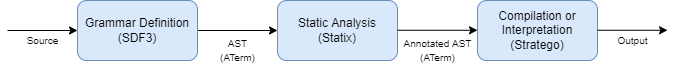
\includegraphics[width=\textwidth]{img/spoofax-p.png}}
  \caption{The Spoofax language workbench pipeline. Source code is parsed using SDF3, analyzed using Statix, then compiled or executed using Stratego.}
  \label{fig:spoofax_pipeline}
\end{figure}

\todo[inline]{improve resolution of spoofax pipeline diagram}

The Spoofax language workbench \cite{Spoofax2021} is a software suite that combines various meta-languages\footnote{A programming language that describes some aspect of another programming language.} and tools to allow users to easily design and implement (domain-specific) programming languages. Beyond parsing, static analysis, and execution, the language workbench is capable of automatically generating various IDE features including syntax highlighting, inline error markers, go-to-definition, hover annotations, and more. A standalone plugin for the Eclipse IDE providing these features can be automatically generated from a Spoofax language project.\\

The most recent stable version of Spoofax, as of the time of writing, is Spoofax 2 \cite{KatsV10}. However, work has been ongoing on Spoofax 3, which retains the same meta-languages and pipeline setup, but integrates this pipeline using PIE \cite{KonatSEV19}, a framework for incrementalizing build tasks. Using PIE, various aspects of Spoofax 3 gain support for incremental compilation "for free", leading to considerable performance gains in both the language development process, as well as the performance of the artifacts produced by the workbench. All projects discussed in this paper, particularly Tim and Dynamix, have been integrated directly into Spoofax 3.\\

The Spoofax language workbench consists of a family of meta-languages that each describe an aspect of a programming language. These meta-languages are often declarative and inspired by academic work, such that it is easy for users to get started if they are familiar with the programming languages academic field. Creating a new language using the Spoofax language workbench amounts to defining each section of the "compiler pipeline" using the appropriate meta-langauge. \Cref{fig:spoofax_pipeline} shows the current compiler pipeline for use in Spoofax. We briefly discuss each step in more detail.

\subsection{Syntax definition and parsing}
\label{sec:spoofax_parsing_aterm}
The natural first part of a language workbench is the ability to declare a grammar for the language. For this purpose, Spoofax offers the Syntax Definition Formalism 3 (SDF3) meta-language \cite{Amorim2019}. Using SDF3, a user is able to declare both lexical and context-free syntax productions for their language. From this declaration, SDF3 generates a scannerless parser with support for error recovery, a pretty-printer, and a syntax highlighter \cite{AmorimV20}.\\

\Cref{fig:sdf3_example} shows an example of an SDF3 definition for a simple arithmetic language. Two lexical sorts are defined, \texttt{INT} and \texttt{ID} which represent an integer literal and variable identifier respectively. A single context-free sort is defined, \texttt{Exp}, which represent an arbitrary expression. The distinction between lexical and context-free sorts determines is similar to that between grammar productions and lexical tokens in other parsers, and mainly determines the way in which the resulting value is represented in the AST (a lexical production yields a string of its contents, whereas a context-free production produces a tuple containing its subterms).\\

The \texttt{LAYOUT} syntax-production on line 5\todo{check/fix line numbers} is used to allow implicit layout between terms in context-free productions. Without this declaration, an expression such as \texttt{1 + 2} would be rejected as invalid. This may be surprising since the syntax for addition is defined with explicit spaces surrounding the \texttt{+} token. Indeed, SDF3 treats this declaration as \texttt{Exp LAYOUT? '+' LAYOUT? Exp}, and only uses the formatting supplied by the language author for the generated pretty-printer. \\

\todo[inline]{remove next paragraph in favor of being more brief and merging it in the previous paragraph?}
The grammar in \cref{fig:sdf3_example} is ambiguous: the expression \texttt{1 + 2 * 3} can be parsed as either \texttt{(1 + 2) * 3} or \texttt{1 + (2 * 3)}. This is resolved through the use of the \textbf{\texttt{context-free priorities}} section (line 25-26). Here, we explicitly state that the division and multiplication operators should bind more tightly than the addition and subtraction operators. Within the same precedence level, each operator is marked as left-associative by annotating its group with \texttt{left:}. The \texttt{\{bracket\}} production in line 15 allows for brackets to be used to explicitly enforce order of operations. The pretty-printer generated by SDF3 will only include these brackets in the output if they are necessary.\\

\begin{figure}
  \begin{sdf3*}{firstline=3,firstnumber=1}
module start

lexical sorts INT ID
lexical syntax
  INT = [1-9] [0-9]*
  ID = [A-Za-z] [A-Za-z0-9]*
  LAYOUT = [\ \n\r\t]

context-free sorts Exp
context-free syntax
  Exp = <(<Exp>)> {bracket}
  Exp.Add = <<Exp> + <Exp>> {left}
  Exp.Sub = <<Exp> - <Exp>> {left}
  Exp.Mul = <<Exp> * <Exp>> {left}
  Exp.Div = <<Exp> / <Exp>> {left}

  Exp.Var = <<ID>>
  Exp.Int = <<INT>>

  Exp.Let = <let <ID> = <Exp> in <Exp>>

context-free priorities
  {left: Exp.Mul Exp.Div} > {left: Exp.Add Exp.Sub} > {Exp.Let}
  \end{sdf3*}
  \caption{A simple SDF3 grammar for an arithmetic language that supports variable bindings.}
  \label{fig:sdf3_example}
\end{figure}

The parser generated by SDF3 ouputs an \ac{AST} in the \acf{ATerm}. This format originated in the ASF+SDF formalism \cite{DHP:1996}, a precursor to the Spoofax language workbench. It is a simple data transfer format that supports strings, integers, lists, tuples, tagged tuples (constructors), and annotations. The grammar for the ATerm format can be seen in \cref{gr:aterm}. \acp{ATerm} are used pervasively across the Spoofax language workbench and are supported as data format in all Spoofax meta-languages. \Cref{fig:sdf3_example_parse_output} shows an example of the parsing output for a simple program using the grammar defined in \cref{fig:sdf3_example}.\\

\begin{figure}
  \centering
  \begin{subfigure}{.35\textwidth}
    \centering
    \begin{mat}
let x = 10 in
  let y = 20 in
    let z = x + y in
      (10 + x) * y / z
    \end{mat}
  \end{subfigure}\hfill%
  \begin{subfigure}{.585\textwidth}
    \centering
    \begin{statix*}{firstline=5,lastline=20,firstnumber=1}
module main

rules
  foo(
Let(
  "x",
  Int("10"),
  Let(
    "y",
    Int("20"),
    Let(
      "z",
      Add(Var("x"), Var("y")),
      Div(
        Mul(Add(Int("10"), Var("x")), Var("y")),
        Var("z")
      )
    )
  )
)
  ).
    \end{statix*}
  \end{subfigure}
  \caption{An example expression in the arithmetic language declared in \cref{fig:sdf3_example}\protect\footnotemark. The parsed \ac{AST} in \ac{ATerm} format as produced by the generated parser can be seen on the right.}
  \label{fig:sdf3_example_parse_output}
\end{figure}

\begin{grammar}[The grammar for the \ac{ATerm} data representation format.][][gr:aterm]
  \firstcase{\prodname{term}}{\prodname{int literal}}{Integer literal}
  \otherform{\prodname{string literal}}{String literal}
  \otherform{\prodname{identifier}\textbt{(}\prodname{terms}\textbt{)}}{Constructor}
  \otherform{\textbt{[}\prodname{terms}\textbt{]}}{List literal}
  \otherform{\textbt{[}\prodname{terms}\textbt{]}}{Tuple literal}
  \otherform{\prodname{term}\textbt{\{}\prodname{terms}\textbt{\}}}{Annotated term}\\

  \firstcase{\prodname{terms}}{\epsilon}{}
  \otherform{\prodname{term}}{}
  \otherform{\prodname{term}\textbt{, }\prodname{terms}}{}\\

  \firstcase{\prodname{int literal}}{\texttt{'-'? [1-9] [0-9]*}}{}
  \firstcase{\prodname{string literal}}{\textbt{" }\prodname{string char}\textbt{* "}}{}
  \firstcase{\prodname{identifier}}{\texttt{[A-Za-z] [A-Za-z0-9.\_-]*}}{}
\end{grammar}

\todo{ensure footnote on correct page}
\footnotetext{The syntax highlighting in this snippet is exactly the syntax highlighting that SDF3 automatically generates using the grammar definition.}

Spoofax will automatically derive an \textit{algebraic signature} from all SDF3 declarations. Such a signature dictates the exact structure that an \ac{ATerm} expression can take such that it is a valid AST\footnote{Here, valid \ac{AST} means that it is an \ac{AST} that can be produced by the parser (i.e. it has a lexical equivalent), and not necessarily that this \ac{AST} is valid according to the static and dynamic semantics of the language.}. These signatures are used by various other meta-languages in the Spoofax language workbench to provide better static analysis features. \Cref{fig:sdf3_example_signature} shows the signature for the example grammar in both formal and Spoofax syntax formats.\\

% For some reason this "centers" the algebraic signature and the statix signature.
\newsavebox{\sdfsignaturebox}
\begin{lrbox}{\sdfsignaturebox}\begin{minipage}{.45\textwidth}
\begin{statix*}{firstline=3,firstnumber=1}
module main

signature
  sorts
    INT = string
    ID = string
    Exp

  constructors
    Add : Exp * Exp -> Exp
    Sub : Exp * Exp -> Exp
    Mul : Exp * Exp -> Exp
    Div : Exp * Exp -> Exp
    Var : ID -> Exp
    Int : INT -> Exp
    Let : ID * Exp * Exp -> Exp
\end{statix*}
\end{minipage}
\end{lrbox}

\begin{figure}
  \centering
  \begin{subfigure}{.45\textwidth}
    \centering
    \usebox{\sdfsignaturebox}
  \end{subfigure}\hfill%
  \begin{subfigure}{.5\textwidth}
    \centering
    $$ S = \{\texttt{INT}, \texttt{ID}, \texttt{Exp}\} $$
    \begin{equation*}
    \begin{aligned}
    \Sigma = \{ \; & \texttt{Add} : \texttt{Exp} \times \texttt{Exp} \to \texttt{Exp}, \\
                  & \texttt{Sub} : \texttt{Exp} \times \texttt{Exp} \to \texttt{Exp}, \\
                  & \texttt{Mul} : \texttt{Exp} \times \texttt{Exp} \to \texttt{Exp}, \\
                  & \texttt{Div} : \texttt{Exp} \times \texttt{Exp} \to \texttt{Exp}, \\
                  & \texttt{Var} : \texttt{ID} \to \texttt{Exp}, \\
                  & \texttt{Int} : \texttt{INT} \to \texttt{Exp}, \\
                  & \texttt{Let} : \texttt{ID} \times \texttt{Exp} \times \texttt{Exp} \to \texttt{Exp} \; \}
    \end{aligned}
    \end{equation*}
  \end{subfigure}
  \caption{The algebraic signature for the grammar in \Cref{fig:sdf3_example}. Left shows the signature of the grammar defined in the Statix meta-language, right shows the grammar in equivalent formal term algebra notation. The left source is automatically derived from the grammar definition by SDF3 as part of the compilation process.}
  \label{fig:sdf3_example_signature}
\end{figure}

Other features that SDF3 offers include the ability to specify layout constraints for grammar productions (often crucial for languages that have significant whitespace such as Python and Haskell) and automatic error recovery and placeholder insertion (needed for robust autocomplete). For more information on SDF3 and parsing within the Spoofax language workbench, the reader is invited to consult the relevant academic work, particularly the work by Visser et al. across various papers \cite{KatsV10a, Spoofax2021, Amorim2019, AmorimV20,KallebergV07, WachsmuthKV14}.

\subsection{Static analysis with constraint solvers}
\label{sec:spoofax_constraint}
The current meta-language used for static analysis in the Spoofax workbench is Statix \cite{AntwerpenPRV18}. Statix is a declarative language that performs static analysis through the use of constraints. A Statix specification consists of a set of declarative rules that specify constraints that should hold for a program to be valid. If the Statix logic solver can find a solution for which all constraints hold for a given input \ac{AST}, a program is considered well-typed. Name binding correctness is asserted through the use of \textit{scope graphs} \cite{TUD-SERG-2015-009}, although their exact semantics are beyond the scope of this paper. The reader is referred to the work by van Antwerpen et al. \cite{TUD-SERG-2015-009,AntwerpenPRV18,VanAntwerpen2016} should they be interested in their exact workings. \\

\Cref{fig:stx_example} shows an example typing rule in both formal notation and Statix syntax. The \texttt{typeOfExpression} rule and $\Gamma \vdash v : \texttt{T}$ notation are equivalent, in that they both describe the relationship between an expression and its type. Within the \textit{head} of the Statix rule, the \texttt{Div(a, b)} node is pattern-matching on exactly the \ac{ATerm} that is output by the parser. Indeed, all values in Statix (including the \texttt{INT()} term) are \acp{ATerm}. Using the signatures generated by SDF3 (see \cref{sec:spoofax_parsing_aterm}, \cref{fig:sdf3_example_signature}), the Statix meta-language can statically ensure that these pattern-matching operations are valid.\\

Beyond simply indicating whether some input \ac{AST} is valid according to the Statix specification, the Statix solver also allows users to attach \textit{properties} to arbitary AST nodes. These properties are arbitrary \ac{ATerm} values and can later be read from outside Statix. Common properties used in Statix specifications are the \texttt{ref} and \texttt{type} properties, which represent the declaring node and the type of a node respectively. The Spoofax language workbench has built-in support for reading the values of these two properties to provide editor services such as hover hints and go-to-definition. An example of the \texttt{type} annotation, as well as the tooltip generated as a result, can be seen in \cref{fig:stx_property_example}. It is worth noting that both the \texttt{type} and \texttt{ref} properties are simply conventions. A user is able to assign arbitrary properties to a property, and can read these values from other meta-languages within the Spoofax language workbench.

\begin{figure}
  \centering
  \begin{subfigure}{.55\textwidth}
    \centering
    \begin{statix*}{firstline=3,firstnumber=1}
module main

rules
  typeOfExpression(s, Div(a, b)) = INT() :-
    typeOfExpression(s, a) == INT(),
    typeOfExpression(s, b) == INT().
    \end{statix*}
  \end{subfigure}\hfill%
  \begin{subfigure}{.45\textwidth}
    \centering
    \begin{prooftree}
    \AxiomC{$\Gamma \vdash a : \texttt{INT}$}
    \noLine
    \UnaryInfC{$\Gamma \vdash b : \texttt{INT}$}
    \RightLabel{T-Division}
    \UnaryInfC{$\Gamma \vdash a \mathbin{/} b : \texttt{INT}$}
    \end{prooftree}
  \end{subfigure}
  \caption{An example typing rule for integer division in both Statix notation and formal notation. Here \texttt{s} and $\Gamma$ are analogous and correspond to the context in which the expression appears. Other rules, such as the type of an integer literal, are omitted.}
  \label{fig:stx_example}
\end{figure}

\begin{figure}
  \centering
  \begin{subfigure}{.55\textwidth}
    \centering
    \begin{statix*}{firstline=3,firstnumber=1,highlightlines={5}}
module main

rules
  typeOfExpression(s, n@Div(a, b)) = INT() :-
    typeOfExpression(s, a) == INT(),
    typeOfExpression(s, b) == INT(),
    @n.type := INT().
    \end{statix*}
  \end{subfigure}\hfill%
  \begin{subfigure}{.40\textwidth}
    \centering
    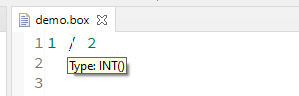
\includegraphics{img/stx_hover_example.png}
  \end{subfigure}
  \caption{An example showing the ability to attach properties to nodes in Statix. The highlighted line (left) sets the \texttt{type} property on the AST node representing the division expression. This value is later read by Spoofax to provide editor services such as hover information (right).}
  \label{fig:stx_property_example}
\end{figure}

\subsection{Transformations with Stratego}
\label{sec:spoofax_transform}
Finally, we will briefly discuss the Stratego transformation language \cite{Visser05-SCAM}. Unlike SDF3 or Statix, Stratego is more of a general imperative programming language centered around the concept of transformations, instead of a (hyper-specialized) meta-language. As a result, it generally functions as a general purpose language that, while traditionally used for interpreteration or compilation at the end of the Spoofax pipeline, may also appear between other stages to perform intermediate transformations.\\

An example of a simple Stratego program can be seen in \cref{fig:str_example}. Pattern-matching is performed on input terms, with matches transformed accordingly. The data format in use for Stratego is again the \ac{ATerm} format, with additional static analysis provided using the algebraic signature automatically derived from the SDF3 grammar.\\

\begin{figure}
  \begin{stratego*}{firstline=3,firstnumber=1}
module start

rules
  fold = innermost(fold-term)

  fold-term: Add(Int(a), Int(b)) -> Int(<addS> (a, b))
  fold-term: Sub(Int(a), Int(b)) -> Int(<subtS> (a, b))
  fold-term: Mul(Int(a), Int(b)) -> Int(<mulS> (a, b))
  fold-term: Div(Int(a), Int(b)) -> Int(<divS> (a, b))

  fold-term: Eq(Int(a), Int(a)) -> Int("1")
  fold-term: Eq(Int(a), Int(b)) -> Int("0") where not(<eq> (a, b))
  \end{stratego*}
  \caption{A simple Stratego program that performs constant folding in an arithmetic language. The \texttt{fold} strategy will apply the \texttt{fold-term} strategy until a fixpoint is reached.}
  \label{fig:str_example}
\end{figure}

\begin{figure}
  \begin{stratego*}{firstline=3,firstnumber=1}
module start

imports
  statix/api

rules
  compile-expr: n@Add(a, b) -> <compile-int-addition> (a, b)
    where a := <stx-get-ast-analysis> n; INT() := <stx-get-ast-type(|a)> n
  
  compile-expr: n@Add(a, b) -> <compile-string-concatenation> (a, b)
    where a := <stx-get-ast-analysis> n; STRING() := <stx-get-ast-type(|a)> n
  \end{stratego*}
  \caption{Many Spoofax meta-languages expose Stratego APIs. Here, the result of a Statix analysis is used to emit integer addition or string concatenation based on the type of the expression.}
  \label{fig:str_stx_example}
\end{figure}

Due to its general nature, many Spoofax features and meta-languages offer a Stratego API. This allows Stratego strategies to interact with other parts of the Spoofax workbench, such as the ability to query the results of static analysis. Consider the example in \cref{fig:str_stx_example}, which uses Statix APIs to distinguish between integer addition and string concatenation, both of which are syntactically represented as \texttt{Add(a, b)}.\\

We will further discuss Stratego and its semantics when we introduce the mini-Stratego case study in \cref{ch:case_studies}. Readers interested in learning more about Stratego and its term rewriting paradigm are encouraged to read the appropriate work by Visser et al. \cite{KallebergV07,Visser05-SCAM}.

\section{Dynamic semantics in Spoofax}
\label{sec:background_spoofax_dynamics}
\todo[inline]{rename section/something with history?}
As already briefly alluded to, Dynamix is not the first attempt at adding dynamic semantics support to the Spoofax language workbench. In fact, several projects, including some under the Dynamix name, predate the work done in this thesis.\\

The first effort at implementing dynamic semantics in the Spoofax language workbench was the DynSem meta language \cite{VerguNV15}. DynSem was conceived with goals similar to Dynamix, but was intentionally designed to mimic the notation often used by big-step operational semantics. The DynSem compiler converts such a specification into an interpreter for the language written in Java. An example of a DynSem specification can be seen in \cref{fig:dynsem_example}. We further discuss DynSem as part of the related work section in \cref{ch:related_work}.\\

\begin{figure}
  \begin{dynsem*}{firstline=3,firstnumber=1}
module start

rules
  Lit(s) --> NumV(parseI(s)).

  Plus(e1, e2) --> NumV(addI(i1, i2))
  where
    e1 --> NumV(i1);
    e2 --> NumV(i2).

  Ifz(NumV(ci), e1, e2) --> v
  where
    case ci of {
      0 => e1 --> v
      otherwise => e2 --> v
    }.
  \end{dynsem*}
  \caption{An example of a specification written using the DynSem meta-language \cite{VerguNV15}. The \texttt{-->} "arrow" is intended to be analogous to a Kahn-style big-step evaluation relation. }
  \label{fig:dynsem_example}
\end{figure}

One of the main problems with DynSem\todo{check with andrew if this is right} was that certain language constructs were hard, or even impossible, to represent in the language. Especially non-linear control flow, such as exceptions and generators, require non-trivial boilerplate in virtually every rule. Additionally, the generated interpreter is not particularly performant. While this performance has been greatly increased in follow-up work by Vergu et al. \cite{VerguV18}, they note that the generated interpreter still performed a factor of 4 slower than a hand-written interpreter for the same language. As a result of these two main drawbacks, the DynSem language saw little use within the Spoofax workbench and was eventually deprecated.\\

In an effort to remedy these issues, the Dynamix meta-language\footnote{Not to be confused with the Dynamix language presented in this paper. With the exception of this section, the term Dynamix will always refer to the language presented in this paper.} was conceived as part of Chiel Bruin's master's thesis \cite{Bruin2020}. Inspired by DynSem, the Dynamix language was conceived as a dynamic specification meta-language compatible with the semantics of the "Roger" target language, introduced in the same thesis. Unfortunately, the Roger language and corresponding FrameVM did not see any future use beyond Bruin's thesis.\todo{mention brams thesis?}\\

Despite this, the Dynamix language seemed promising. In late 2020, Eelco Visser and Andrew Tolmach started exploratory work on "Dynamix V2". The intent was to retain most of the Dynamix language, but to compile to a new continuation-based target language. If the resulting target language was able to be efficiently compiled or interpreted, this approach could resolve the runtime performance issues that DynSem suffered from. DynSem's other main problem, that of control flow, could also be resolved by using continuations, as evident from Bruin's work.\\

The Dynamix language discussed in this thesis\footnote{Dynamix as presented in this paper should really be called Dynamix v2.5. However, since the version of Dynamix designed by Bruin never made it into the Spoofax language workbench, the Dynamix presented in this paper is the first publicly usable iteration of the meta-language. In order to avoid potential confusion for Spoofax users, we decided that it would be more appropriate to call the language Dynamix, without a version number.} is a spiritual successor to these efforts by Visser and Tolmach. Many components were revamped in order to generalize their experimental prototype to a large array of languages and programming paradigms, and to fully integrate the resulting product in the Spoofax language workbench. The remainder of this thesis discusses these efforts and shows that the resulting meta-language is indeed capable of resolving many of DynSem's original issues.
% !TEX root = ../document.tex

\chapter{\label{ch:design}Designing a \acs{DSL} for runtime semantics}
\todo{better chapter title?}

% The ultimate goal\todo{bleh} of this thesis is to design and implement a new \ac{DSL} that functions as a method of defining the runtime semantics of a programming language. This \ac{DSL} should be expressive enough to implement a large variety of languages, while also providing a method of turning a language specification into a program (either an interpreter or a compiler) capable of executing the language.\\

In this chapter, we discuss a set of features that a \ac{DSL} for runtime semantics should conform to in order to be a minimally viable product. We also discuss what its position is compared to other parts of a language definition (e.g. the grammar and static semantics), how it may want to interact with the results of these stages, and what features would help widen the range of source languages the \ac{DSL} might be applicable for.\\

Within this chapter, we use the term \textbf{source language} to refer to the language under compilation (i.e. the language for which a runtime semantics specification is written). Unless otherwise specified, the term \textbf{\ac{DSL}} refers to the \ac{DSL} for dynamic specification whose design we are considering. The term \textbf{rule} refers to the runtime semantics for a single source language construct (e.g. a single rule may define the behavior of integer multiplication). The term \textbf{specification} refers to the set of all runtime semantics \textbf{rule}s (for the source language) written in the \ac{DSL}.

\section{Visualizing our objectives}
\label{sec:design_requirements}
\todo{do not number this subsection maybe?}
\todo[inline]{we need to state this somewhere, but not entirely sure if a new subsection is the right place to do it. Moving it to before the start of the sections reads better but requires us to be more brief(?). Other parts of this chapter need to be touched up to consider the intro either way, and refer back to the design goals}
Before we start the design process of our \ac{DSL}, we must first consider exactly \textit{what} we desire to achieve. Even if we do not yet have any idea how exactly our \ac{DSL} will manifest itself, we can use the desired outcome as a way to guide the design process. To do so, let us first restate the design objectives we briefly discussed in the introduction (\cref{ch:introduction}) and elaborate on them. \\

\subsubsection*{Easy to use for language designers}
\todo{better goal title}
Where possible, our \ac{DSL} should have some form of resemblance to existing formalisms and conventions for dynamic specifications. Such resemblances will help users familiarize themselves by giving them the ability to associate constructs within the \ac{DSL} with concepts and approaches that they already understand.\todo{additionally it might help since existing literature would become (partially) applicable?}

\subsubsection*{Applicable to a wide variety of language paradigms}
Our \ac{DSL} should offer abstractions capable of handling a large number of programming paradigms. Users should be able to implement their language of choice without being limited by a lack of \ac{DSL} features. This is not to say that \textit{every} language should be supported, nor that every language should be efficiently executed. Instead, features within the \ac{DSL} should be chosen and designed in a way where they do not unnecessarily limit the general applicability of the \ac{DSL}.

\subsubsection*{Focus on runtime performance}
\todo{better goal title}
Specifications written in our \ac{DSL} should lead to a program capable to executing source language programs with speeds within an order of magnitude compared to a manual (optimized) implementation. Desiring a fast runtime for a language should be a valid motivator for writing a language specification using our \ac{DSL}.\todo{this paragraph is bad, reword}

\subsubsection*{Direct integration with the Spoofax language workbench}
Our \ac{DSL} should have a tight and idiomatic integration with other meta-languages in the Spoofax language workbench. Users should be able to easily write dynamic specifications for their existing Spoofax projects, without overhauling parts of their projects. The design and behavior of the language should, where applicable, be consistent with other Spoofax meta-languages to allow for easier adoption.

\section{The anatomy of a formal runtime semantics specification}
\label{sec:design_anatomy}

\begin{figure}
  \begin{prooftree}
    \AxiomC{$ G,E,S \vdash e_1 : str(n_1, s_1), S_1, \_ $}
    \noLine
    \UnaryInfC{$ G,E,S_1 \vdash e_2 : str(n_2, s_2), S_2, \_ $}
    \noLine
    \UnaryInfC{$ v = str(n_1 + n_2, s_1 || s_2) $}
    \RightLabel{\;\;\;\textsc{[Str-Concat]}}
    \UnaryInfC{$G,E,S \vdash e_1 + e_2 : v, S_2, \_ $}
  \end{prooftree}
  \begin{prooftree}
    \AxiomC{$ G,E,S \vdash e_1 : int(i_1), S_1, \_ $}
    \noLine
    \UnaryInfC{$ G,E,S_1 \vdash e_2 : int(i_2), S_2, \_ $}
    \noLine
    \UnaryInfC{$ v = int(i_1 + i_2) $}
    \RightLabel{\;\;\;\textsc{[Int-Addition]}}
    \UnaryInfC{$G,E,S \vdash e_1 + e_2 : v, S_2, \_ $}
  \end{prooftree}
  \caption{Examples of the runtime semantics for string concatenation and integer addition in formal notation for the ChocoPy language. Adapted from the ChocoPy reference manual by Padhye et al. \cite{PadhyeSH19}.}
  \label{fig:chocopy_semantics_example}
\end{figure}

\newcommand{\jvar}[1]{\textit{\texttt{#1}}}
\newcommand{\jop}[1]{\texttt{#1}}

\begin{figure}
  \subsection*{EvaluateStringOrNumericBinaryExpression(\jvar{leftOperand}, +, \jvar{rightOperand})}
  \begin{itemize}
    \item Let \jvar{lref} be the result of evaluating \jvar{leftOperand}.
    \item Let \jvar{lval} be ? \jop{GetValue}(\jvar{lref}).
    \item Let \jvar{rref} be the result of evaluating \jvar{rightOperand}.
    \item Let \jvar{rval} be ? \jop{GetValue}(\jvar{rref}).
    \item Let \jvar{lprim} be ? \jop{ToPrimitive}(\jvar{lval}).
    \item Let \jvar{rprim} be ? \jop{ToPrimitive}(\jvar{rval}).
    \item If \jop{Type}(\jvar{lprim}) is String or \jop{Type}(\jvar{lprim}) is String, then
    \begin{itemize}
      \item Let \jvar{lstr} be ? \jop{ToString}(\jvar{lprim}).
      \item Let \jvar{rstr} be ? \jop{ToString}(\jvar{rprim}).
      \item Return the string-concatenation of \jvar{lstr} and \jvar{rstr}.
    \end{itemize}
    \item Note: at this point it must be a numeric operation.
    \item Let \jvar{lnum} be ? \jop{ToNumeric}(\jvar{lval}).
    \item Let \jvar{rnum} be ? \jop{ToNumeric}(\jvar{rval}).
    \item \textit{[NaN and infinite cases omitted]}
    \item Assert: \jvar{lnum} and \jvar{rnum} are both finite.
    \item If \jvar{lnum} is $ - 0_{\mathbb{F}} $ and \jvar{rnum} is $ -0_{\mathbb{F}} $, return $ - 0_{\mathbb{F}} $.
    \item Return $ \mathbb{F}(\mathbb{R}(\jvar{lnum}) + \mathbb{R}(\jvar{rnum})) $.
  \end{itemize}
  \caption{Examples of the runtime semantics for string concatenation and number addition in the JavaScript programming language. Certain steps are omitted for the sake of brevity. Adapted from the ECMAScript 2023 language specification \cite{ecma1999262}.}
  \label{fig:javascript_semantics_example}
\end{figure}

We will start our design process by taking a look at existing formal specifications of several programming languages. Doing so allows us to derive a minimal set of features needed to replicate these specifications in our new \ac{DSL}, while at the same time giving us a general idea of what the syntax of the \ac{DSL} may look like. In particular, we will consider the formal specifications of the plus (\texttt{+}) operator, responsible for both numerical addition and string concatenation. This operation was chosen for several reasons: it is a common and well-understood operation, it involves different behavior based on the types of its sub-expressions, and one has to consider the underlying data storage (such as the bit-width of the numeric types and the wrapping behavior when addition may overflow) when defining the operation.\\

The languages specifications that we will consider are those of the ChocoPy programming language \cite{PhadyeSH19-SPLASHE}, as well as the ECMAScript specification for the JavaScript programming language \cite{ecma1999262}. These were chosen for several reasons: they vary in notational style (the ChocoPy specification uses big-step denotational semantics\footnote{Big-step denotational semantics, also known as natural semantics or Kahn-style semantics, are a notational style for dynamic semantic specifications due to Gilles Kahn \cite{Kahn87:0}. In big-step semantics, the notation $\rho \vdash E \Rightarrow \alpha$ indicates that the expression $E$, when evaluated in the environment $\rho$, yields the value $\alpha$.}, the ECMAScript specification uses natural language), they represent different language designs (ChocoPy is statically typed, JavaScript is dynamically typed), and they target different platforms (ChocoPy is intended to be compiled to RISC-V assembly, JavaScript is traditionally interpreted). \Cref{fig:chocopy_semantics_example,fig:javascript_semantics_example} show formal specifications of the plus operator for ChocoPy and JavaScript, respectively.\\

The ChocoPy specification of the plus operator (\cref{fig:chocopy_semantics_example}) is described using formal notation. The \textit{store} parameter $S$, which represents the values of all locations currently in use by the program, is explicitly specified as an input and output parameter to each operation. Since the evaluation of $e_2$ uses store $S_1$, it must logically be evaluated after $e_1$. As a result, if evaluating $e_1$ had side-effects, those effects must be visible when $e_2$ is evaluated. The specification also considers the underlying data representation of the values. String values (\texttt{str}) are defined to carry both the length and the contents of the string as separate fields, and the concatenation explicitly notes that the resulting string length is the sum of the individual lengths. How exactly integers are stored, and how overflow should be handled, is mentioned elsewhere in the ChocoPy manual \cite{PadhyeSH19}: integers are signed 32-bit values, and the behavior when this addition overflows is undefined\footnote{"Undefined behavior" is a common term in formal language specifications and indicates a complete lack of obligations on a particular implementation of the language when such behavior occurs. Returning an arbitrary value, crashing the program, or even shutting down the computer would all be behaviors consistent with the specification.}.\\

The ECMAScript specification of the plus operator (\cref{fig:javascript_semantics_example}) uses natural language instead of formal notation to describe the operation. Here, unlike the ChocoPy specification, there is no explicit "state-threading". Instead, it is implicitly assumed that operations are performed in the order in which they are listed, and that any underlying changes to the program environment as a result of these operations are reflected in the next step. Indeed, the current environment in which the expressions are evaluated ($ G, E, S $ in the ChocoPy specification) is implicitly inherited from the environment that contained the addition expression. The specific data representations of both numbers and strings, as well as the exact behavior of string-concatenation and the $\mathbb{F}$ and $\mathbb{R}$ operators, are defined elsewhere in the specification.\\

Both specifications perform \textit{conditional} behavior to determine whether to apply numeric or string addition. For the ECMAScript specification, this branching is explicitly done at runtime: the type of the operands is derived only after they are both evaluated. This is a natural choice for JavaScript: it is impossible to always statically predict the runtime types of expressions due to its dynamically-typed nature\footnote{It should be noted that even through JavaScript is dynamically-typed, advanced JavaScript engines are able elide the vast majority of type checks through a combination of static and runtime analysis. This elision does not conflict with the specification, since it is only performed in situations where the engine is able to prove that it is safe to do so.}. The ChocoPy specification is more ambiguous in how a specific rule is selected. It is clear that the premises of the \textsc{[Str-Concat]} and \textsc{[Int-Addition]} rules are disjoint (after all, a value cannot be both an integer and a string at the same time), but there is no explicit process described for exactly \textit{when} to select a rule. Since ChocoPy is statically typed, a compiler that unconditionally emits either string concatenation or integer addition code based on the types involved would adhere to the specification. However, an implementation that performed this check at runtime would be equally valid (since the ChocoPy specification imposes no specific restrictions on both the data representation of values and the time complexity of the addition operation). This shows an interesting aspect of formal specifications for programming languages: their primary aim is to describe \textit{how} programs are executed, but this description does not necessarily translate to the most optimal\footnote{Generally, a language implementation is considered more optimal if it runs faster. However, different requirements may call for a different definition of optimal (e.g. consider a lightweight implementation meant for low-power electronics, which may favor simplicity over performance).} implementation.\\

Based on the two discussed specification examples, we can derive the following categories of features that our \ac{DSL} should support. These give a baseline set of requirements that the designed \ac{DSL} should conform to in order to replicate the ChocoPy and ECMAScript specifications. We justify these requirements by higlighting the appropriate sections in the discussed examples.\todo{interesting enough? reword paragraph?}

\begin{itemize}
  \item \textbf{Static rule selection}. The \ac{DSL} should be able to offer some deterministic method for selecting which rule(s) are applicable for any specific language construct. It should be possible to indicate that one rule applies to the multiplication operator, whereas another applies to the subtraction operator.
  \begin{itemize}
    \item In the formal notation used by the ChocoPy specification, the applicable rules for some expression $ e $ are the ones for which $ G, E, S \vdash e : v, S', \_ $ appears in the conclusion. The ECMAScript specification uses natural language to indicate that a binary expression should defer to the appropriate \texttt{Evaluate\hspace{0pt}String\hspace{0pt}Or\hspace{0pt}Numeric\hspace{0pt}Binary\hspace{0pt}Expression} implementation.
  \end{itemize}
  \item \textbf{Runtime conditional behavior}. A rule in the \ac{DSL} should be able to perform conditional behavior based on values derived at runtime, for situations where an applicable rule cannot be selected statically. It should be possible to only conditionally evaluate (sub-)expressions.
  \begin{itemize}
    \item The ECMAScript specification performs conditional behavior at runtime to differentiate between numerical addition and string concatenation. The discussed ChocoPy examples do not perform any conditional behavior. Conditional evaluation is essential to in order to be able to specify branching behavior (e.g. if-then-else statements, loops).
  \end{itemize}
  \item \textbf{Clear ordering of operations}. It should be unambigious in what order operations are evaluated in a \ac{DSL} rule, and how these operations affect the surrounding state of the program.
  \begin{itemize}
    \item The ChocoPy example explicitly threads stores by using $ S_n $. The ECMAScript specification implicitly specifies that operations are executed in exactly the listed order. Both specifications explicitly require the left-hand side of the addition operator to be evaluated before the right-hand side.
  \end{itemize}
  \item \textbf{Access to primitive operations}. It should be possible to express "primitive" operations in the \ac{DSL}, such as arithmetic operations, I/O operations, and interacting with the operating system.
  \begin{itemize}
    \item Both the ChocoPy and ECMAScript specification use the addition operator in its mathematical sense. This is a primitive operation, as it cannot be expressed using other operations within the language. Such operations must therefore be provided by the runtime platform (e.g. ChocoPy addition might be performed using the \texttt{add} RISC-V instruction), and exposed by the \ac{DSL}.
  \end{itemize}
  \item \textbf{Appropriate control over data representation}. A rule in the \ac{DSL} should be able to control the runtime data representation of values within the language, to a certain degree. A user should be able to specify representation-dependent options, such as the bit-width of integer values and their wrapping behavior. A user should be able to form composite values, such as tuples, records, or structs.
  \begin{itemize}
    \item Neither the ChocoPy nor the ECMAScript specification fully specifies the runtime data representation of its values, opting to allow the implementation to choose an appropriate representation. However, both specifications put requirements on the data representation of certain values: integers in ChocoPy \textbf{must} be 32-bit signed, and numbers in ECMAScript must be 64-bit IEEE 754-2019 \cite{8766229} double-precision floating point numbers.
  \end{itemize}
\end{itemize}

%   - Compilation process should involve "compilation"/translation of the source program based on the rules.
%     - Effectively meta-interpreting the source language (all possible paths).
%     - Meta-interpreting requires some output language/data format.

\section{From specification to evaluation}
So far, we have only discussed the definition aspects of a runtime semantics \ac{DSL}. An equally important part is the ability to transform a specification into some method of running the source programs. Without this capability, the \ac{DSL} would simply be yet another notation for runtime semantics. In this section, we discuss several different approaches for using a specification written in our \ac{DSL} to automatically run source language programs. \\

Broadly speaking, we've established that a formal specification essentially acts as a list of instructions to perform when a certain language construct should be executed. These instructions interact with the runtime environment of the program (such as its memory, variables) and dictate which constructs should be evaluated next, in what order, and how their results are used. Logically, this means that "running" a specification with some source program as input effectively involves repeatedly selecting the appropriate rule to apply, then evaluating all steps for that rule until the program reaches termination. There are multiple ways of doing this, each with their own set of upsides and downsides. The most common solutions include:

\todo[inline]{revise/review naming of these approaches}
\begin{itemize}
  \item \textbf{A \ac{DSL} interpreter.} A single program takes both a specification and a source program AST as parameters. The interpreter selects the appropriate "entry rule" for the input AST, then (recursively) executes each instruction in the rule.
  \item \textbf{Automatic interpreter/compiler generation.} The specification is used to generate a specialized interpreter or compiler for the target language. The resulting program can be used to directly run or compile source programs.
  \item \textbf{A \ac{DSL} meta-interpreter.} A single program takes both a specification and a source program AST as parameters. The interpreter selects the appropriate "entry rule" for the input AST, then traverses the program, substituting each source language construct with the appropriate instructions from the specification. The resulting output is a language-agnostic set of instructions corresponding to the input program, which can subsequently be compiled or interpreted directly.
\end{itemize}

\noindent Let us briefly discuss each of these approaches and consider their strengths and weaknesses in more detail. 

\subsubsection*{Direct interpretation} Arguably the simplest approach is to write a direct interpreter for the \ac{DSL}. This involves using an input (desugared, type checked) \ac{AST} to guide which rule(s) should be executed, with each specification instruction executed in-order. Since a specification is effectively a formal description of an interpreter for the language, this approach typically is not very performant due to the "nested" interpretation (the interpreter interprets the \ac{DSL}, which in turn interprets the source language). However, this approach is very portable (a single interpreter is capable of running every specification on every source snippet) and generally easy to implement and debug. This is the approach taken by PLT Redex \cite{MatthewsFFF04}  (further discussed in \cref{ch:related_work}).

\subsubsection*{Specialized interpreter/compiler generation} The abstract specification is transpiled\footnote{Source-to-source compilation between two languages of a similar abstraction level.} to a interpreter or compiler in a concrete programming language. The resulting program can be used to directly run source ASTs. This is often a more performant approach to running the specification, as the overhead of the meta-language largely disappears. An example of a project that uses this approach is the DynSem \cite{VerguNV15} dynamic specification language, which automatically translates a specification into an AST-based interpreter running on the Java virtual machine (we further discuss DynSem in \cref{ch:related_work}). The final performance of the generated interpreter or compiler depends largely on how it is implemented. For example, subsequent work by Vergu et al. \cite{VerguV18} on the same DynSem framework demonstrated performance increases of up to 15x by improving the generated interpreter.

\subsubsection*{Meta-interpretation} The final approach we will discuss is that of \textit{meta-interpretation}. This approach lends itself from the observation that, due to the nature of a dynamic specification, a program where every source construct is replaced with the body of the appropriate dynamic specification rule behaves exactly the same. After all, the behavior of the source program is defined through the specification. As we will discuss later, this is the approach used by Dynamix for executing source programs. An example of this approach can be seen in \cref{fig:meta_interpretation}.

The meta-interpretation technique is quite similar to symbolic execution\footnote{A method of executing a program in an abstract manner, where every possible behavior of the source program is considered. Originally introduced by James C. King \cite{King76:0}, it is a common analysis technique used for testing, verifying, and debugging programs. Unlike symbol execution, meta-interpretation does not consider symbolic values and only evaluates all (potential) program control flow.}, but unlike symbolic execution it only considers rule selection and recursive rule invocation based on the input source language \ac{AST}. Any operations that require runtime state (such as access to memory, variables, or conditional jumps) are deferred. The resulting output is effectively the \textit{application} of the specification on the specific input. One could also consider this process as \textit{compiling} a source AST to a collection of \ac{DSL} instructions. For the example in \cref{fig:meta_interpretation}, observe that the numeric literal \texttt{10} has been inlined into the declaration for \texttt{LetDeclaration}, but that all memory operations have been retained.\todo{might make more sense to talk about treating the spec as rewrite rules instead of this weird analogue to symbolic execution}

The benefit to the meta-interpretation technique is that it is able to generically transform every source language for which a specification exists into a singular language-agnostic format. The resulting format can be directly interpreted or compiled into a target program. Since this language-agnostic format is common between all possible specifications and source languages, it is comparatively simpler to efficiently compile or run the program (compared to the interpreter generation approach, which cannot make any assumptions about the language which it is interpreting).

\begin{figure}
  \begin{plain}
on Program(stmts):
  - execute each stmt in `stmts` sequentially

on LetDeclaration(name, value):
  - let `v` be the result of executing `value`
  - assert: there is no global variable `name`
  - assign `v` to the global variable `name`

on IntLiteral(value):
  - yield the 32-bit signed representation of `value`

on Print(value):
  - let `v` be the result of executing `value`
  - let `str` be the result of converting `v` to a string representation
  - output `str` to standard output, followed by a newline character (0x0A, '\n')
  \end{plain}
  \begin{plain}
let x = 10;
print x;
  \end{plain}
\begin{plain}
let `v` be the 32-bit signed integer 10
assign `v` to the global variable `x`
let `v1` be the value of the global variable `x`
let `str` be the string representation of `v1`
output `str` to standard output, followed by a newline character (0x0A, '\n')
\end{plain}
  \caption{A dynamic specification (top) and input program (middle) for a fictional language. The bottom program represents the result of meta-interpreting the source program, yielding a new program where every source language construct has been replaced with the appropriate instructions in the specification language.}
  \label{fig:meta_interpretation}
\end{figure}

\section{Considering control flow}
\label{sec:design_control_flow}
One aspect of a language specification we have so far largely glossed over is that of control flow. While \cref{sec:design_anatomy} considers control flow from the aspect of evaluation order, we have yet to discuss constructs like conditionals, loops, and exceptions. With our intent to provide a \ac{DSL} capable of describing a large number of source languages, we must make an effort to support most, if not all, of these constructs in an easy manner.

\subsection{Control flow in existing specifications}
The natural approach to implementing control flow in a dynamic specification is by simply abstracting it through conditional rule selection. Consider the example in \cref{fig:chocopy_conditional_example}. The method for selecting the appropriate rule that applies to the while statement is used as a method to perform control-flow: the conditional check implicitly introduced by the rule selection is used to perform the conditional behavior that a while loop must perform at the start of each iteration. A similar definition can be used to conditionally evaluate statements, such as an if-then-else expression.\\

\begin{figure}
  \begin{prooftree}
    \AxiomC{$ G,E,S \vdash e_1 : bool(true), S_1, \_ $}
    \RightLabel{\;\;\;\textsc{[While-False]}}
    \UnaryInfC{$G,E,S \vdash \texttt{while }  e_1 : b_1 : \_, S_1, \_ $}
  \end{prooftree}
  \begin{prooftree}
    \AxiomC{$ G,E,S \vdash e_1 : bool(false), S_1, \_ $}
    \noLine
    \UnaryInfC{$ G,E,S_1 \vdash b_1 : \_, S_2, \_ $}
    \noLine
    \UnaryInfC{$ G,E,S_2 \vdash \texttt{while } e_1 : b_1 : \_, S_3, \_ $}
    \RightLabel{\;\;\;\textsc{[While-True]}}
    \UnaryInfC{$G,E,S \vdash \texttt{while }  e_1 : b_1 : \_, S_3, \_ $}
  \end{prooftree}
  \caption{Control flow as seen in the ChocoPy reference manual \cite{PadhyeSH19}. The appropriate rule is chosen based on the evaluation of the condition expression $e_1$. The \textsc{[While-True]} case recurses as a means of performing multiple iterations.}
  \label{fig:chocopy_conditional_example}
\end{figure}

This abstraction becomes much less simple in the presence of statements that can abruptly jump to a different part of the program, such as the \texttt{return} statement. In fact, the ChocoPy reference manual defines another case as part of the while loop semantics, specifically for handling early returns. This case can be seen in \cref{fig:chocopy_conditional_early_return}. The last value in the output triplet, $ R $, indicates the value returned from the function. Every other rule that affects control flow must consider this value, and possibly immediately return it without evaluating the rest of the construct (e.g. a function body must not execute the remaining instructions if an early return is encountered).\\

This approach is manageable if one only needs to support early returns, but it doesn't scale very well\footnote{Perhaps this is the reason why ChocoPy does not support the \texttt{continue} and \texttt{break} constructs.}. The ECMAScript specification \cite{ecma1999262} handles this by wrapping the result of an evaluation inside a \textit{continuation}. This continuation indicates whether execution should continue normally, or whether it should move elsewhere (e.g. because an exception was thrown). The \texttt{?} character prefixed to certain operations in the ECMAScript example discussed earlier (\cref{fig:javascript_semantics_example}) is part of this abstraction: it indicates that if the result of the following function call was an \textit{abrupt completion} (i.e. an exception was thrown), that this result should immediately be propagated upwards without continuing the remainder of the rule.\\

\begin{figure}
  \begin{prooftree}
    \AxiomC{$ G,E,S \vdash e_1 : bool(true), S_1, \_ $}
    \noLine
    \UnaryInfC{$ G,E,S_1 \vdash b_1 : \_, S_2, R $}
    \noLine
    \UnaryInfC{$ R \texttt{ is not } \_ $}
    \RightLabel{\;\;\;\textsc{[While-True-Return]}}
    \UnaryInfC{$G,E,S \vdash \texttt{while }  e_1 : b_1 : \_, S_2, R $}
  \end{prooftree}
  \caption{A specialized case of the while construct as seen in the ChocoPy reference manual \cite{PadhyeSH19}. This case aborts control flow if some statement in the body of the loop performed an early return.}
  \label{fig:chocopy_conditional_early_return}
\end{figure}

This approach is powerful enough to handle a wide range of control flow features, including early returns, loop breaking, generators, asynchronous functions and exceptions. However, it comes at the cost of additional complexity in the specification (e.g. the possibility of an exception must be handled in every rule that can indirectly cause one) and has substantial overhead if a language implementation directly implements control flow in this manner. Clearly, both the usability and performance of our \ac{DSL} would benefit from an alternative implementation for control flow that does not suffer from these issues.

\subsection{Control flow through continuations}
An alternative approach to control flow within a dynamic specification borrows from a technique first described by Strachey and Wadsworth \cite{continuations_mathematical_semantics}. They propose the use of \textit{continuations}\footnote{Continuations were independently conceived by several different computer scientists, but the version used by Strachey et al. originates from the work by Mazurkiewicz \cite{Mazurkiewicz71}. Reynolds's "The Discoveries of Continuations" \cite{Reynolds93} discusses the full origins of the continuation concept.}, an abstract term representing "the meaning of the rest of the program" (Reynolds,  \cite{Reynolds93}), as a method of modeling the mathematical semantics of a programming language with jumps. The core insight is to no longer consider the semantics of each language construct in isolation. As Strachey and Wadsworth put it:

\begin{quote}
The solution to this problem is to abandon the idea of giving the state transformation for each command in isolation. We must define, instead, a semantic function which yields, for every command $\gamma$, in a program, the state transformation which would be produced from there to the end of the program.
\end{quote}

Particularly, we will add an additional parameter to our evaluation relation, indicating the continuation of the expression. This continuation is some abstract representation of a point in the program (e.g. a label or a function) where evaluation should continue after the evaluation relation has completed.\\

Consider the example in \cref{fig:continuation_introduction}. We introduce a new \texttt{continuation} parameter, representing a \textit{label} to which execution\footnote{We use the term execution here, but it is important to consider that this usage of continuations is \textit{only within the dynamic specification}. A specific implementation of the language is not required to use the specific continuation implementation, or even use continuations at all. We use the term execution only because it is convenient to view a dynamic specification as a set of instructions to be followed at runtime.} should jump after the completion of the computation described in the body of the function. For the evaluation of the subexpressions \texttt{leftOperand} and \texttt{rightOperand}, we simply indicate that they should continue directly on the next line at the \textsc{AfterLeft} and \textsc{AfterRight} labels. Conceptually, this transformation just makes the implicit returning behavior of functions (i.e. that they jump back to the callee directly after the call expression) explicit.\\

\begin{figure}
  \subsection*{EvaluateStringOrNumericBinaryExpression(\jvar{leftOperand}, +, \jvar{rightOperand}\hl{, }\jvar{\hl{continuation}})}
  \begin{itemize}
    \item Evaluate \jvar{leftOperand}\hl{ with continuation label \textsc{AfterLeft}.}
  \end{itemize}
\hl{\textsc{\small AfterLeft(\textit{\texttt{lref}})}:}
  \begin{itemize}
    \item Let \jvar{lval} be ? \jop{GetValue}(\jvar{lref}).
    \item Evaluate \jvar{rightOperand}\hl{ with continuation label \textsc{AfterRight}.}
  \end{itemize}
\hl{\textsc{\small AfterRight(\textit{\texttt{rref}})}:}
  \begin{itemize}
    \item Let \jvar{rval} be ? \jop{GetValue}(\jvar{rref}).
    \item \textit{[several steps omitted]}
    \item Let \jvar{result} be $ \mathbb{F}(\mathbb{R}(\jvar{lnum}) + \mathbb{R}(\jvar{rnum})) $.
    \item \hl{Jump to \textit{\texttt{continuation}} with value \textit{\texttt{result}}.}
  \end{itemize}
  \caption{A rewritten version of the ECMAScript addition example from \cref{fig:javascript_semantics_example} that uses continuation labels for control flow. The highlighted sections indicate changes needed to support continuations. Text in \textsc{Small Caps} indicates a definition or reference to a continuation label.}
  \label{fig:continuation_introduction}
\end{figure}

The real benefit of a continuation-based approach becomes clear when we perform control flow. \Cref{fig:continuation_early_return} contains a fictional implementation of the evaluation of statements in ECMAScript. In the case that the statement is a sole expression, it is directly evaluated, with execution continuing at \textsc{AfterExpressionStatement}. This simply discards the result of the expression, then jumps to \jvar{continuation} (which presumably represents the next statement). However, if the statement represents an early return, we instead execute the expression with the continuation label \textsc{\$ReturnFromFunction} (assumed to have been defined when we entered the current function). This simple change has big consequences: because we never jump to \jvar{continuation}, control flow never continues "past" the return statement. The callee never has to consider an early return, as it won't even continue execution in the case where such an early return has occurred.\\

\begin{figure}
  \subsection*{EvaluateStatement(\jvar{statementType}, \jvar{subExpression}, \jvar{continuation})}
  \begin{itemize}
    \item If \jvar{statementType} is \texttt{ExpressionStatement}:
    \begin{itemize}
      \item Evaluate \jvar{subExpression} with continuation label \textsc{AfterExpressionStatement}.
    \end{itemize}
    \item If \jvar{statementType} is \texttt{ReturnStatement}:
    \begin{itemize}
      \item Evaluate \jvar{subExpression} with continuation label \textsc{\$ReturnFromFunction}.
    \end{itemize}
    \item \textit{[other cases omitted]}
  \end{itemize}
\textsc{AfterExpressionStatement(\textit{\texttt{discarded}}):}
  \begin{itemize}
    \item Jump to \jvar{continuation}.
  \end{itemize}
  \caption{Using continuations to implement the \texttt{return} statement. We assume that the continuation label \textsc{\$ReturnFromFunction} has been defined earlier and that it implements the process of returning a value from a function.}
  \label{fig:continuation_early_return}
\end{figure}

Other control flow can be implemented in a similar way. For example, exceptions can be handled by designating a \textsc{\$HandleException} continuation. Throwing an exception can then be implemented by virtue of simply continuing execution at this label, instead of the supplied continuation. Analogously, the \texttt{break} statement might be implemented by defining a continuation label positioned after the body of the loop.\\

\todo[inline]{the following paragraph needs a bit less opinion and a bit more segue into finalizing the section}
As far as I am aware, no current language specification makes use of continuations as an abstraction over control flow, despite their promising abilities. Perhaps the notational overhead of continuations, or an increase in cognitive complexity when reading the specification, makes them an unattractive abstraction. This is not too surprising, given that the main benefit of modeling control flow through continuations is that it allows for more efficient execution (if one were to directly convert a specification to a language implementation), and that it allows for better defined mathematical semantics, neither of which are usually priorities for a formal language specification. \\

However, a continuation based approach to control flow lends itself excellently to our \ac{DSL}. Efficient compilation of programs that use continuations is a well-understood problem\footnote{The book "Compiling with Continuations" by Andrew W. Appel \cite{Appel1992} is an excellent introduction to techniques for compilation using \acf{CPS}.}, and a structural approach to continuations aided by effective static analysis will relieve some of the cognitive complexity of working with continuations.

%   - How does one allow complex non-linear control flow?
%     - Abstract over control-flow itself!
%     - Natural result: CPS
%   - TODO: Discuss holy terms here? Should prob wait until Tim is introduced?

\section{A minimum-viable feature set}
\label{sec:design_features}

\todo{See content}
%   - What kind of capabilities should a dynamic specification language support?
%     - Support for "native" operations implemented on a lower level than target language itself (primitives!)
%     - Support for being able to interface with the constraint analyzer/static analysis
%     - Support for complex non-linear control flow
%     - Nice to have:
%       - Type system/verification of operations where possible
%       - Multi-file setup
\chapter{Design choices}

\todo[inline]{We need a place somewhere to go from floaty hypothetical land to concrete facts land. Right now, we've discussed several approaches for how one might design a DSL, and we've introduced Spoofax. However, we've not yet said how any of this directly relates to Dynamix. If we want the next chapters to be Tim and Dynamix, we'll likely need to make it slightly more concrete before we jump into it. Maybe illustrate the Dynamix architecture/pipeline first? Although this does make it weird as we'll effetively split up the Dynamix chapter into two separate chapters.}

\todo[inline]{This is also probably a good place to talk about the fact that Dynamix was (partially)inherited from earlier work by Eelco, Andrew.}
% !TEX root = ../document.tex

\chapter{\label{ch:tim}The Tim intermediate representation}

Before we discuss the Dynamix language, we must first take a detour and discuss the language that it targets. As briefly alluded to in \cref{ch:design}, Dynamix converts a language specification into a runnable program through the technique of \textit{meta-interpretation}\todo{better name} (see \cref{sec:design_evaluation}). However, instead of directly converting a source program into a sequence of Dynamix runtime instructions, we instead transform the source program into a more specialized \acf{IR} containing only the subset of Dynamix instructions that would actually be executed at runtime. By doing so, we can independently work on the Dynamix meta-language and the interpreter or compiler for the output \ac{IR}.\\

The specific \ac{IR} that Dynamix compiles\footnote{For the remainder of this thesis, whenever we use the term compilation within the context of Dynamix, it will refer to the process of meta-interpreting a Dynamix specification on a given input source. The name "compilation" is not inappropriate for this process. After all, Dynamix translates the input source to a lower-level specialized instruction set.} to is a new Spoofax meta-language called Tim\footnote{The name Tim originates from Target InterMediate language.}. Tim is a human-readable language with a relatively low level of abstraction that is designed to use \acf{CPS} (this choice coincides with the choice to use continuations as abstractions for control flow in Dynamix). Its grammar and semantics are largely inspired by the \ac{CPS} \ac{IR} used by the Standard ML compiler and described in Andrew W. Appel's book, Compiling with Continuations \cite{Appel1992}.\\

In this chapter, we discuss Tim's grammar (\cref{sec:tim_grammar}), dynamic semantics (\cref{sec:tim_runtime_semantics}), static semantics (\cref{sec:tim_static_semantics}), the Tim interpreter (\cref{sec:tim_interpreter}) and how it may be extended or improved upon in future work (\cref{sec:tim_future}).

\todo[inline]{perhaps a little introduction section to tim with examples here?}

\section{Design and grammar}
\label{sec:tim_grammar}
Tim as an intermediate representation centers around \acf{CPS} as a way of modeling control flow. As dicussed in chapter \ref{ch:design}, using a continuation-based approach to control flow modeling in a dynamic specification language is a natural way of allowing a wide-range of control flow while at the same time being able to take advantage of well-known compilation and optimization strategies available to \ac{CPS}-based languages.\\

Let us first discuss the grammar of Tim. Despite Tim being an \ac{IR} (and therefore not a language directly designed to be used by users), it has a properly defined syntax. This representation allows a user to inspect the output of a Dynamix compilation, write code directly in the target representation (which may be useful if Dynamix does not expose the necessary facilities to do so), and will also help us consider the semantics of Tim without needing to resort to abstract representations of terms. Note that this is unlike the \ac{CPS} \ac{IR} from "Compiling with Continuations" \cite{Appel1992} that Tim is based on, which only considers the algebraic signature of the IR and has no formal syntax definition. \Cref{gr:tim} shows the full grammar for the Tim \ac{IR}.\\

\begin{grammar}[The grammar of the Tim intermediate representation.][][gr:tim]
  \firstcase{\prodname{program}}{\prodname{exp}}{}\\

  \firstcase{\prodname{exp}}{\prodname{value}\textbt{(}\prodname{values}\textbt{)}}{Function tail call}
  \otherform{\textbt{\#}\prodname{primitive}\textbt{(}\prodname{values}\textbt{) => }\prodname{identifier}\textbt{; }\prodname{exp}}{Primitive call}
  \otherform{\textbt{\#}\prodname{primitive}\textbt{(}\prodname{values}\textbt{)}}{Primitive tail call}
  \otherform{\textbt{if \#}\prodname{primitive}\textbt{(}\prodname{values}\textbt{) then }\prodname{exp}\textbt{ else }\prodname{exp}}{Conditional primitive}
  \otherform{\textbt{fix \{ }\prodname{funs}\textbt{ \} in }\prodname{exp}}{Function definition}
  \otherform{\textbt{let }\prodname{bindings}\textbt{ in }\prodname{exp}}{Let definition}\\
  
  \firstcase{\prodname{value}}{\prodname{int literal}}{Integer literal}
  \otherform{\prodname{string literal}}{String literal}
  \otherform{\prodname{identifier}}{Variable reference}\\

  \firstcase{\prodname{values}}{\epsilon}{}
  \otherform{\prodname{value}}{}
  \otherform{\prodname{value}\textbt{, }\prodname{value}}{}\\

  \firstcase{\prodname{fun}}{\textbt{fun }\prodname{identifier}\textbt{(}\prodname{identifiers}\textbt{) = }\prodname{exp}}{}\\

  \firstcase{\prodname{funs}}{\epsilon}{}
  \otherform{\prodname{fun}}{}
  \otherform{\prodname{fun}\textbt{ }\prodname{funs}}{}\\

  \firstcase{\prodname{binding}}{\prodname{identifier}\textbt{ = }\prodname{value}}{}\\

  \firstcase{\prodname{bindings}}{\epsilon}{}
  \otherform{\prodname{binding}}{}
  \otherform{\prodname{binding}\textbt{, }\prodname{bindings}}{}\\

  \firstcase{\prodname{identifier}}{\texttt{[a-zA-Z\_\$] [a-zA-Z0-9\_\$-]*}}{}\\

  \firstcase{\prodname{identifiers}}{\epsilon}{}
  \otherform{\prodname{identifier}}{}
  \otherform{\prodname{identifier}\textbt{, }\prodname{identifiers}}{}\\

  \firstcase{\prodname{int literal}}{\texttt{'-'? [1-9] [0-9]*}}{}
  \firstcase{\prodname{string literal}}{\textbt{" }\prodname{string char}\textbt{* "}}{}
  \firstcase{\prodname{primitive}}{\texttt{[A-Za-z0-9\_+*/-]+}}{}
\end{grammar}

As you may note, Tim's grammar is very simple. At a first glance, one may think that this simplicity interferes with the design goals for Dynamix and Tim; after all, we desire for them to be generic enough to support a large variety of source languages. However, as we will discuss later (see also \cref{ch:case_studies}), just the small set of operations in Tim are enough to represent a wide range of source language paradigms.\\

Part of this expressiveness comes from the concept of primitive calls. Primitives are Tim's approach to compiler intrinsics: functions whose body is implemented directly by the Tim compiler or runtime. Through primitives, Tim can expose operations like integer addition and access to composite data structures without the need to introduce explicit new grammar for these actions. Tim also diverges from the \ac{IR} used in "Compiling with Continuations" in this aspect: while both \acp{IR} have the concept of primitive operations, the \ac{IR} used in Appel's book limits the available primitive operations to a fixed set, whereas primitives in Tim are allowed to be any valid identifier. Similarly, operations that have their own constructs in Appel's \ac{IR}, such as \texttt{RECORD} and \texttt{SWITCH}, are represented using primitive (tail) calls in Tim instead.\\

Primitives come in three forms: calls, tail calls, and conditionals. Primitive tail calls usually perform some form of control flow and as a result must appear in the tail call position. Non-tail calls to primitives do not break the \ac{CPS} expectation that calls must be in a tail call position: while primitives may look like function calls, their body is directly inlined and non-tail call primitives are not allowed to perform control flow. Conditional primitives\footnote{You may wonder why Tim has a separate if-then-else conditional primitive construct when such a construct can also be implemented by simply passing two separate continuations to a primitive tail call. The reason is simply because it allows Dynamix to have an if-then-else construct that directly correlates with a Tim construct. It has the added benefit of making Tim programs slightly more readable.} are only valid in if-then-else expressions and allow for conditional branching based on a compiler-implemented test (e.g. integer equality). An annotated example of a Tim program that uses primitives can be seen in \cref{fig:tim_example}. \\

One particular property of the Tim grammar, as well as its corresponding algebraic signature, is that it is \textit{\ac{CPS}-by-construction}. That is, the design of the grammar automatically enforces that certain properties of the \ac{CPS} hold for any well-formed Tim term. In particular, the grammar enforces that calls are always in the tail position, and that arguments to calls are atomic values (i.e. literals or variable references, but not complex sub-expressions).\\

\todo{tail call or tail call? green book uses both, wikipedia says tail call}
Enforcing proper tail call behavior is done by carefully modeling how multiple expressions combine. Instead of a sequencing operator (e.g. \texttt{exp ',' exp}) or a flat block statement (e.g. \texttt{'\{' exp* '\}'}), each expression in Tim directly embeds the next expression. The only expressions that do not specify their subsequent expression are function calls and primitive tail calls. This trivially makes them the final expression in a sequence, and hence enforces that every call is a tail call. Note that this property also means that every expression \textit{must} end in a tail call: it is simply not possible to terminate a sequence of expressions with anything other than a (primitive) tail call.\\

Enforcing that expressions (and function calls in particular) do not contain complex sub-expressions is done simply by making these a different sort. \textit{Values} are defined to be solely the expressions that directly yield a value: integer literals, string literals, and vriable references. Only values may be passed to function and primitive calls.\\

\begin{figure}
  \begin{tim}
// Functions within a fix block can refer to each other.
fix {
  fun main() =
    #print("Please input a number: ") => tmp0;

    // primitive tail call with two distinct continuations
    #read-number(onValidNumber, onInvalidNumber)
    
  fun onValidNumber(num) =
    // even simple arithmetic instructions are primitives
    #int-add(num, 1) => out;
    #print(out) => tmp0;
    #exit() // exit program
    
  fun onInvalidNumber() =
    #print("Invalid number entered.") => tmp0;
    main() // retry
} in
  main()
  \end{tim}
  \caption{A simple annotated Tim program that reads an integer value, increments it by one, and outputs it. If an invalid value is entered, an error message is displayed. Primitive calls are used to invoke I/O operations and arithmetic.}
  \label{fig:tim_example}
\end{figure}

\todo[inline]{or perhaps show some more tim examples here?}

\section{Dynamic semantics}
\label{sec:tim_runtime_semantics}
We will deviate a bit from the usual order in which languages are defined, and focus on the runtime semantics of Tim first. The reason why we will consider the runtime semantics first will become clear once we discuss the typing rules in \cref{sec:tim_operations}.\\

\subsection{Notation}
We formally define the runtime semantics of Tim through Kahn-style big-step operational semantics \cite{Kahn87:0}. To do so, let us first define some notation.\\

The store, $S$, is a mapping from variable names to their concrete value. Since Tim variables are immutable once created, we do not require a seperate environment and store. In order to still facilitate mutable values, we provide the heap, $H$, which functions as a mapping from address to value. The heap is not exposed to any Tim language constructs, but it may be freely accessed by the implementations of certain primitives. We use the syntax $S' = S[x \mapsto y]$ (respectively $H' = H[x \mapsto y]$) to extend $S$ with a new mapping from $x$ to $y$, yielding the store $S'$ (respectively heap $H'$). If $ S $ already contained a mapping for $ x $, it is \textit{shadowed} by the new value $ y $ in $ S' $, but remains accessible in $ S $. The syntax $S' = S[x/y]$ (respectively $H' = H[x/y]$) represents a store where the value bound to $ x $ is \textit{replaced} with $ y $. The syntax $ S[x] $ retrieves the value bound to $x$ in store $S$. \\

Runtime values are denoted as $v = X(a_1, a_2, ..., a_n)$. Here $X$ is the \textit{discriminant}, indicating the type of the value. The content of the data is included in the arguments $a_1$ through $a_n$. The core Tim language has three different runtime values: $int(i)$, $str(s)$ and $func(S, args, body)$. For the function runtime value, the associated $S$ indicates the environment that the function closes over. Primitives can return additional data types, prefixed with \texttt{\#}. These data values are opaque to core Tim constructs and can only be handled by primitives that support these data types.\\

Since Tim uses \acf{CPS}, we will define an expression term as yielding a continuation $ C $. Such a continuation may either be $ cont(S, e) $, indicating that execution should continue at expression $ e $ with store $ S $, or $ exit() $, indicating that execution should stop. As we will see later, we can define execution of a program as repeatedly evaluating continuations until we reach the $ exit() $ term.\\

We will use two different relations to define the behavior of Tim. For values\footnote{With values, we mean the "value" term type from the Tim grammar, indicating an atomic expression. When needed, we'll use the terms "value term" and "runtime value" to disambiguate between the two.}, we'll use the notation $ S, H \vdash e : v $ to indicate that the value term $ e $ evaluates to the runtime value $ v $ within the store $ S $ and heap $ H $. Since value terms cannot have side effects, we do not have to consider any changes to $ S $ or $ H $. For expressions, we use the notation $ S, H \vdash e \rightarrow C, H' $ to indicate that evaluating the expression $ e $ yields a continuation $ C $. We do not need to yield an $ S' $, as the continuation already contains the store to be used for subsequent expressions.

\subsection{Semantics of the core language}
With the notation defined, we can discuss the semantics of the Tim core\footnote{We define "Tim core" to be the parts of the Tim language that are statically defined, i.e. anything but the behavior of primitives.} language. Let us start simple by defining the behavior of values. String and integer literals directly convert to their runtime equivalents. For variables, we perform a lookup in the store.

\begin{prooftree}
  \AxiomC{}
  \RightLabel{\textsc{V-Int Literal}}
  \UnaryInfC{$S, H \vdash i : int(v)$}
\end{prooftree}

\begin{prooftree}
  \AxiomC{}
  \RightLabel{\textsc{V-String Literal}}
  \UnaryInfC{$S, H \vdash s : str(s)$}
\end{prooftree}

\begin{prooftree}
  \AxiomC{$v = S[x]$}
  \RightLabel{\textsc{V-Variable Reference}}
  \UnaryInfC{$S, H \vdash x : v$}
\end{prooftree}

With values out of the way, let us tackle the expressions. A \texttt{let}-binding simply extends the store with a new name for a value. Newly defined variables are only visible in the body, and not in subsequent bindings of the same let.\todo{make a comment here about how we could've also returned $cont(H_n, b)$, but we're reserving that syntax for actual continuations?}

\begin{prooftree}
  \AxiomC{$S, H \vdash e_1 : v_1$}
  \noLine
  \UnaryInfC{$S_1 = S[x_1 \mapsto v_1]$}
  \noLine
  \UnaryInfC{$S, H \vdash e_2 : v_2$}
  \noLine
  \UnaryInfC{$S_2 = S_1[x_2 \mapsto v_2]$}
  \noLine
  \UnaryInfC{\vdots}
  \noLine
  \UnaryInfC{$S, H \vdash e_n : v_n$}
  \noLine
  \UnaryInfC{$S_n = S_{n-1}[x_n \mapsto v_n]$}
  \noLine
  \UnaryInfC{$S_n, H \vdash b \rightarrow C, H'$}
  \RightLabel{\textsc{E-Let}}
  \UnaryInfC{$S, H \vdash \textbt{let } x_1 = e_1, x_2 = e_2, ..., x_n = e_n\textbt{ in } b \rightarrow C, H'$}
\end{prooftree}

\texttt{fix} expressions are used to declare functions. Functions declared within the same \texttt{fix} block are allowed to refer to each other, as well as any variables declared in a higher scope (they \textit{capture} their scope). \todo{better notation that does not require recursive usage of S'?}\todo{better notation that isn't so W I D E}

\begin{prooftree}
  \AxiomC{$f_1 = func(S', args_1, body_1)$}
  \noLine
  \UnaryInfC{$f_2 = func(S', args_2, body_2)$}
  \noLine
  \UnaryInfC{\vdots}
  \noLine
  \UnaryInfC{$f_n = func(S', args_n, body_n)$}
  \noLine
  \UnaryInfC{$S' = S[name_1 \mapsto f_1, name_2 \mapsto f_2, ..., name_n \mapsto f_n]$}
  \noLine
  \UnaryInfC{$S', H \vdash b \rightarrow C, H'$}
  \RightLabel{\textsc{E-Fix}}
  \UnaryInfC{$S, H \vdash \textbt{fix \{ } \textbt{fun } name_1 \textbt{(} args_1 \textbt{) = } body_1 \cdots \textbt{fun } name_n \textbt{(} args_n \textbt{) = } body_n \textbt{ \} in } b \rightarrow C, H'$}
\end{prooftree}

The (tail) call expression can be used to call functions. For a call to be valid, it must resolve to a value of type $ func $ with a matching number of arguments. We substitute the argument names into a new environment based on the captured environment from the function, then return a continuation value indicating that execution should continue at the body of the called function.

\begin{prooftree}
  \AxiomC{$S, H \vdash id : func(S_f, args, body)$}
  \noLine
  \UnaryInfC{$ S, H \vdash a_1 : v_1 $}
  \noLine
  \UnaryInfC{$ S, H \vdash a_2 : v_2 $}
  \noLine
  \UnaryInfC{\vdots}
  \noLine
  \UnaryInfC{$ S, H \vdash a_n : v_n $}
  \noLine
  \UnaryInfC{$S_f' = S_f[args_1 \mapsto v_1, args_2 \mapsto v_2, ..., args_n \mapsto v_n]$}
  \noLine
  \UnaryInfC{$C = cont(S_f', body)$}
  \RightLabel{\textsc{E-Tail Call}}
  \UnaryInfC{$S, H \vdash id \textbt{(} a_1, a_2, ..., a_n \textbt{)} \rightarrow C, H $}
\end{prooftree}

The primitive tail call is very similar, but we defer the next continuation as well as the resulting heap to the implementation of the primitive. It is an error to call a primitive that is not defined. We discuss the semantics of several primitives in \cref{subsec:tim_primitive_semantics}.

\begin{prooftree}
  \AxiomC{$ S, H \vdash a_1 : v_1 $}
  \noLine
  \UnaryInfC{$ S, H \vdash a_2 : v_2 $}
  \noLine
  \UnaryInfC{\vdots}
  \noLine
  \UnaryInfC{$ S, H \vdash a_n : v_n $}
  \noLine
  \UnaryInfC{$ C, H' = \textsc{TailPrimitive}(H, \textbt{\#}$id$, v_1, v_2, ..., v_n) $}
  \RightLabel{\textsc{E-Primitive Tail Call}}
  \UnaryInfC{$S, H \vdash \texttt{\#} id \textbt{(} a_1, a_2, ..., a_n \textbt{)} \rightarrow C, H' $}
\end{prooftree}

Non-tail calls to primitives are similar, but instead of returning a continuation return a value directly. Note that even non-tail call continuations are allowed to change the heap.

\begin{prooftree}
  \AxiomC{$ S, H \vdash a_1 : v_1 $}
  \noLine
  \UnaryInfC{$ S, H \vdash a_2 : v_2 $}
  \noLine
  \UnaryInfC{\vdots}
  \noLine
  \UnaryInfC{$ S, H \vdash a_n : v_n $}
  \noLine
  \UnaryInfC{$ v, H_1 = \textsc{Primitive}(H, \textbt{\#}$id$, v_1, v_2, ..., v_n) $}
  \noLine
  \UnaryInfC{$ S' = S[x \mapsto v]$}
  \noLine
  \UnaryInfC{$ S', H_1 \vdash e \rightarrow C, H_2 $}
  \RightLabel{\textsc{E-Primitive Call}}
  \UnaryInfC{$S, H \vdash \texttt{\#} id \textbt{(} a_1, a_2, ..., a_n \textbt{) => } x \textbt{; } e \rightarrow C, H_2 $}
\end{prooftree}

Finally, conditional primitives are simply invoke the primitive function and branch based on the result of this invocation. It should be noted that the $true$ and $false$ in the semantics here are simply indications on which branch should be taken, with no particular requirements on exactly how these values are represented.

\begin{prooftree}
  \AxiomC{$ S, H \vdash a_1 : v_1 $}
  \noLine
  \UnaryInfC{$ S, H \vdash a_2 : v_2 $}
  \noLine
  \UnaryInfC{\vdots}
  \noLine
  \UnaryInfC{$ S, H \vdash a_n : v_n $}
  \noLine
  \UnaryInfC{$ b, H_1 = \textsc{ConditionalPrimitive}(H, \textbt{\#}$id$, v_1, v_2, ..., v_n) $}
  \noLine
  \UnaryInfC{$ e =\left\{\def\arraystretch{1.2}\begin{tabular}{@{}l@{\quad}l@{}}
    $e_1$ & if $b$ is $true$ \\
    $e_2$ & if $b$ is $false$
  \end{tabular}\right.$ }
  \noLine
  \UnaryInfC{$ S, H_1 \vdash e \rightarrow C, H_2 $}
  \RightLabel{\textsc{E-Primitive Conditional}}
  \UnaryInfC{$S, H \vdash \textbt{if \#} id \textbt{(} a_1, a_2, ..., a_n \textbt{) then } e_1 \textbt{ else } e_2 \rightarrow C, H_2 $}
\end{prooftree}

\subsection{Executing continuations to completion}
\label{subsec:tim_continuation_iteration}
Now that we know the semantics of individual expressions, let us consider how to execute a Tim program to completion. To execute some program $ p $ (which consists of a top-level expression), we simply iteratively apply the appropriate dynamic semantics rule to yield a continuation $ C $. If this continuation is $ cont(S', e') $, we re-apply the appropriate rule for $ e' $. We halt once we reach the $ exit() $ continuation. We use the notation $ S, H \vdash e \Rightarrow C $ to indicate this operation, using the double arrow to indicate that we repeatedly apply the relation.

\begin{prooftree}
  \AxiomC{$S, H \vdash e \rightarrow cont(S', e'), H' $}
  \noLine
  \UnaryInfC{$ S', H' \vdash e' \Rightarrow C $}
  \RightLabel{\textsc{E-Program Recurse}}
  \UnaryInfC{$S, H \vdash e \Rightarrow C $}
\end{prooftree}

\begin{prooftree}
  \AxiomC{$S, H \vdash e \rightarrow exit(), \_ $}
  \RightLabel{\textsc{E-Program Exit}}
  \UnaryInfC{$S, H \vdash e \Rightarrow exit() $}
\end{prooftree}

\todo[inline]{elaborate more here? give an example of these rules being applied?}

\subsection{Semantics of various primitives}
\label{subsec:tim_primitive_semantics}
Now let us discuss the semantics of some of the primitives available to Tim programs. Since Tim offers an \acs{API} for language designers to implement their own primitives, it is impossible to provide an exhaustive list of all primitives and their semantics. Rather, this section is intended as a way to show how primitives may be implemented and how they are capable of significantly extending the features available to Tim programs. Appendix ??\todo{does it?} contains a full list of the semantics for primitives used in the case studies discussed in \cref{ch:case_studies}.\\

\noindent The \texttt{\#exit} primitive is the only way to gracefully terminate execution:

\begin{prooftree}
  \AxiomC{}
  \RightLabel{\textsc{Prim-Exit}}
  \UnaryInfC{$\textsc{TailPrimitive}(H, \textbt{\#exit}) = exit(), H$}
\end{prooftree}

\smallskip

\noindent Simple operations, such as integer addition, \texttt{\#int-add}, are expressed through primitives. But primitives are not limited to only performing a single operation: the \texttt{\#str-add} primitive performs string concatenation, a considerably more complex operation\footnote{An alternative approach would be to expose primitives to convert strings to and from character arrays, and having the user perform the concatenation of the two arrays themselves.}.

\begin{prooftree}
  \AxiomC{}
  \RightLabel{\textsc{Prim-Int Add}}
  \UnaryInfC{$\textsc{Primitive}(H, \textbt{\#int-add}, int(a), int(b)) = int(a + b), H$}
\end{prooftree}

\begin{prooftree}
  \AxiomC{}
  \RightLabel{\textsc{Prim-String Add}}
  \UnaryInfC{$\textsc{Primitive}(H, \textbt{\#str-add}, str(a), str(b)) = str(a || b), H$}
\end{prooftree}

\smallskip

\noindent Conditional primitives such as \texttt{\#int-eq} are implemented by evaluating the conditional and returning either $ true $ or $ false $.

\begin{prooftree}
  \AxiomC{$ b =\left\{\def\arraystretch{1.2}\begin{tabular}{@{}l@{\quad}l@{}}
    $true$ & if $a = b$ \\
    $false$ & otherwise
  \end{tabular}\right.$ }
  \RightLabel{\textsc{Prim-Int Equality}}
  \UnaryInfC{$\textsc{ConditionalPrimitive}(H, \textbt{\#int-eq}, int(a), int(b)) = b, H$}
\end{prooftree}

\smallskip

\noindent Tim variables are immutable. The \texttt{\#ref-new}, \texttt{\#ref-fetch} and \texttt{\#ref-store} primitives allow for (shared) mutable values by allocating a value on the heap, and returning an opaque value that contains a reference to the allocated value, noted as $\#ref(x)$.

\begin{prooftree}
  \AxiomC{$ x = $ new address not occupied in $H$}
  \noLine
  \UnaryInfC{$ H' = H[x \mapsto v] $}
  \noLine
  \UnaryInfC{$ v_h = \#ref(x) $}
  \RightLabel{\textsc{Prim-Ref New}}
  \UnaryInfC{$\textsc{Primitive}(H, \textbt{\#ref-new}, v) = v_h, H'$}
\end{prooftree}

\begin{prooftree}
  \AxiomC{$ v = H[x] $}
  \RightLabel{\textsc{Prim-Ref Fetch}}
  \UnaryInfC{$\textsc{Primitive}(H, \textbt{\#ref-fetch}, \#ref(x)) = v, H$}
\end{prooftree}

\begin{prooftree}
  \AxiomC{$ H' = H[x/v] $}
  \RightLabel{\textsc{Prim-Ref Store}}
  \UnaryInfC{$\textsc{Primitive}(H, \textbt{\#ref-store}, \#ref(x), v) = v, H'$}
\end{prooftree}

\smallskip

\noindent Primitives may also be used to introduce new data structures. The \texttt{\#record-new}, \texttt{\#record-read}, and \texttt{\#record-write} primitives define and use a $\#record$ data structure, which functions as a heap-allocated list of key-value pairs. We use the notation $ r = rec(k_1=v_1, ..., k_n=v_n) $ to construct such a list, $ r[k_1] $ to retrieve the value bound to $ k_1 $ in record $ r $, and $ r[k_x \mapsto v_x] $ to extend $ r $ with a new mapping from $ k_x $ to $ v_x $, possibly shadowing the previous value. It is a runtime error to retrieve a value for an undefined key.

\begin{prooftree}
  \AxiomC{$ x = $ new address not occupied in $H$}
  \noLine
  \UnaryInfC{$ r = rec(k_1 = v_1, k_2 = v_2, ..., k_n = v_n) $}
  \noLine
  \UnaryInfC{$ H' = H[x \mapsto r] $}
  \noLine
  \UnaryInfC{$ v_{out} = \#record(x) $}
  \RightLabel{\textsc{Prim-Record New}}
  \UnaryInfC{$\textsc{Primitive}(H, \textbt{\#record-new}, str(k_1), v_1, str(k_2), v_2, ..., str(k_n), v_n) = r, H'$}
\end{prooftree}

\begin{prooftree}
  \AxiomC{$ r = H[x] $}
  \noLine
  \UnaryInfC{$ v = r[k] $}
  \RightLabel{\textsc{Prim-Record Read}}
  \UnaryInfC{$\textsc{Primitive}(H, \textbt{\#record-read}, \#record(x), str(k)) = v, H$}
\end{prooftree}

\begin{prooftree}
  \AxiomC{$ r = H[x] $}
  \noLine
  \UnaryInfC{$ r' = r[k \mapsto v] $}
  \noLine
  \UnaryInfC{$ H' = H[x/r'] $}
  \RightLabel{\textsc{Prim-Record Write}}
  \UnaryInfC{$\textsc{Primitive}(H, \textbt{\#ref-store}, \#record(x), str(k), v) = v, H'$}
\end{prooftree}

\section{Static semantics}
\label{sec:tim_static_semantics}
Let us now discuss the static semantics for Tim. Just like the \ac{CPS} \ac{IR} from "Compiling with Continuations", Tim is dynamically typed. Variables and function arguments have no statically defined type and be assigned any value, regardless of its type. Tim also has arbitrary primitives, with the ability for a language designer to define their own. As a consequence of this, we cannot perform much in terms of static analysis. In fact, the static semantics specification for Tim only defines the behavior of name binding, which we will discuss in \cref{sec:tim_name_binding}.\\

However, the lack of static typing does not prevent us from making an attempt at performing static analysis. While the formal definition of Tim only includes the name binding rules, I have written an Statix specification for Tim for use within the Spoofax workbench. This specification uses the constraint engine from Statix to infer types of variables in order to statically reject \textit{some} invalid programs. We will discuss this specification in \cref{sec:tim_statix}.

\subsection{Name binding semantics}
\label{sec:tim_name_binding}
Let us define the environment $ O $ as the set of variables in scope. We will then define the judgement $ O \vdash e $ ($ O \vdash v $) to indicate that expression $ e $ (respectively value term $ v $) has valid name bindings with respect to environment $ O $. To extend an environment $ O $ with a new binding $ x $, we use the syntax $ O' = O \cup \{ x \} $. If $ O $ already contained a binding $ x $, it will be \textit{shadowed}, such that any references to $ x $ within $ O' $ refer to the new value (note that the binding within $ O $ remains the original $ x $). We use the shorthand $ O \vdash v_1, v_2, ..., v_n $ to indicate that values $ v_1 $ through $ v_n $ must have valid name binding within the environment $ O $.\\

\Cref{fig:tim_name_binding} lists the full name binding rules for Tim. Generally, language features that introduce new bindings do so by extending their scope, shadowing any previous bindings with the same name. There is only a single namespace for both variables and functions (since functions are first-class values in Tim), and no access visibility modifiers. Within \texttt{fix} and \texttt{let} constructs, names that reside within the same scope (e.g. function names within a \texttt{fix} block, argument names in a single function) must be distinct.

\begin{figure}
  \begin{prooftree}
    \AxiomC{}
    \RightLabel{\textsc{B-Int Literal}}
    \UnaryInfC{$ O \vdash i $}
  \end{prooftree}
  \begin{prooftree}
    \AxiomC{}
    \RightLabel{\textsc{B-String Literal}}
    \UnaryInfC{$ O \vdash s $}
  \end{prooftree}
  \begin{prooftree}
    \AxiomC{$ x \in O $}
    \RightLabel{\textsc{B-Variable Reference}}
    \UnaryInfC{$ O \vdash x $}
  \end{prooftree}
  \begin{prooftree}
    \AxiomC{$ O \vdash v_0, v_1, ..., v_n $}
    \RightLabel{\textsc{B-Call}}
    \UnaryInfC{$ O \vdash v_0\textbt{(}v_1, v_2, ..., v_n\textbt{)} $}
  \end{prooftree}
  \begin{prooftree}
    \AxiomC{$ O \vdash v_1, v_2, ..., v_n $}
    \noLine
    \UnaryInfC{$ O' = O \cup \{ x \} $}
    \noLine
    \UnaryInfC{$ O' \vdash e $}
    \RightLabel{\textsc{B-Primitive Call}}
    \UnaryInfC{$ O \vdash \textbt{\#}primitive\textbt{(}v_1, v_2, ..., v_n\textbt{) => }x\textbt{; } e $}
  \end{prooftree}
  \begin{prooftree}
    \AxiomC{$ O \vdash v_1, v_2, ..., v_n $}
    \RightLabel{\textsc{B-Primitive Tail Call}}
    \UnaryInfC{$ O \vdash \textbt{\#}primitive\textbt{(}v_1, v_2, ..., v_n\textbt{)}$}
  \end{prooftree}
  \begin{prooftree}
    \AxiomC{$ O \vdash v_1, v_2, ..., v_n $}
    \noLine
    \UnaryInfC{$ S \vdash e_1 $}
    \noLine
    \UnaryInfC{$ S \vdash e_2 $}
    \RightLabel{\textsc{B-Primitive Conditional}}
    \UnaryInfC{$ O \vdash \textbt{if \#}primitive\textbt{(}v_1, v_2, ..., v_n\textbt{) then } e_1 \textbt{ else }e_2$}
  \end{prooftree}
  \begin{prooftree}
    \AxiomC{$ f_1, f_2, ..., f_n $ distinct}
    \noLine
    \UnaryInfC{$ a_{i,1}, a_{i,2}, ..., a_{i,m} $ distinct for all $ i \in [1, n] $}
    \noLine
    \UnaryInfC{$ O_f = O \cup \{ f_1, f_2, ..., f_n \} $}
    \noLine
    \UnaryInfC{$ O_1 = O_f \cup \{ a_{1,1}, a_{1, 2}, ..., a_{1,m} \} $}
    \noLine
    \UnaryInfC{$ O_1 \vdash b_1 $}
    \noLine
    \UnaryInfC{$\vdots$}
    \noLine
    \UnaryInfC{$ O_n = O_f \cup \{ a_{n,1}, a_{n, 2}, ..., a_{n,m} \} $}
    \noLine
    \UnaryInfC{$ O_n \vdash b_n $}
    \noLine
    \UnaryInfC{$ O_f \vdash e $}
    \RightLabel{\textsc{B-Fix}}
    \UnaryInfC{$ O \vdash \textbt{fix \{ } \textbt{fun } f_1 \textbt{(} a_{1,1}, a_{1,2}, ..., a_{1,m} \textbt{) = } b_1 \cdots \textbt{fun } f_n \textbt{(} a_{n,1}, a_{n,2}, ..., a_{n,m} \textbt{) = } b_n \textbt{ \} in } e $}
  \end{prooftree}
  \begin{prooftree}
    \AxiomC{$ x_1, x_2, ..., x_n $ distinct}
    \noLine
    \UnaryInfC{$ O \vdash e_1 $}
    \noLine
    \UnaryInfC{$ O \vdash e_2 $}
    \noLine
    \UnaryInfC{$\vdots$}
    \noLine
    \UnaryInfC{$ O \vdash e_n $}
    \noLine
    \UnaryInfC{$ O' = O \cup \{ x_1, x_2, ..., x_n \} $}
    \noLine
    \UnaryInfC{$ O' \vdash b $}
    \RightLabel{\textsc{B-Let}}
    \UnaryInfC{$ O \vdash \textbt{let } x_1 = e_1, x_2 = e_2, ..., x_n = e_n\textbt{ in } b$}
  \end{prooftree}
  \caption{The name binding rules for Tim.}
  \label{fig:tim_name_binding}
\end{figure}

\todo[inline]{Is there a good example on static semantics for name binding?}

\subsection{Approximating static analysis with Statix}
\label{sec:tim_statix}
While Tim's design does not lend it well to static analysis beyond name binding, some attempts can be made to infer types of variables and functions based on their declaration sites and usage. In order to aid language designers in debugging their programs, the Tim implementation in the Spoofax language workbench includes a static specification using Statix \cite{AntwerpenPRV18} (see also \cref{sec:spoofax_constraint} for more information on Statix). This specification checks name binding according to the rules discussed in \cref{sec:tim_name_binding}, but it also attempts to type-check variables, function calls, and primitive calls by inferring types of values. This way, the specification acts as a "smoke test"\footnote{A test that checks whether some system at least appears to function properly. Smoke tests are often very coarse grained and assert things like "does the program start without immediately crashing".} that gives users an opportunity to see whether their Tim program has trivial errors. \\

Within the Statix specification for Tim, types of variables are inferred from their assigned values. Since variables are immutable once created, and it is impossible to declare a name without immediately assigning a value to it (with the exception of function arguments), we can directly infer the type of a variable from the type of the value assigned to it. For function arguments, we use the constraint-solving engine to infer the type of an argument from its usage, by assigning it an unconstrained wildcard variable. \cref{fig:tim_statix_inference} shows an example of this inference in action.\\

\todo[inline]{snippet of statix necessary/nice to have here?}

% \begin{figure}
%   \begin{statix*}{firstline=4}
% module foo

% rules
% // declare function argument `name` in scope `s`
% declareFunArg(s, name) = T :-
%   @name.type := T,
%   declareVar(s, name, T). // note: T is intentionally unconstrained

% // declare let-binding in scope `dS`, checking value in scope `s`'
% declareBind(s, dS, TBind(name, val)) :- {T}
%   typeOfTValue(s, val) == T,
%   declareVar(dS, name, T),
%   @name.type := T.
%   \end{statix*}
%   \caption{An excerpt from the Statix specification for Tim. }
%   \label{fig:tim_statix_spec_example}

% example of primitive typings here?
% \end{figure}

\begin{figure}
  \centering
  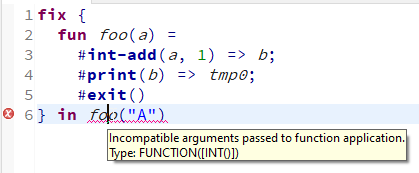
\includegraphics{img/tim_stx_inference.png}
  \caption{Type inference in the Statix specification for Tim. Statix is able to determine that the type of \texttt{a} is an integer based on its usage, and rejects the function call with the wrong argument type.}
  \label{fig:tim_statix_inference}
\end{figure}

There are several drawbacks to the Statix specification that prevent it from becoming a complete static specification for Tim. These drawbacks are also the reason why the language definition for Tim, despite the existence of a complete Statix specification, only formally specifies the name binding rules. In particular, these constraints are the following:\\

\noindent \textbf{Type signatures of primitives must be defined inside the Statix specification.} In order to properly infer types, the Statix specification must know the type signature of each primitive. Since there is no syntax to declare these signatures, they must be directly hardcoded in the specification. As a result, only a select handful of default primitives are supported by the Statix specification.\\

\noindent \textbf{The type system used is (too) simplistic}. In order to avoid specifying a complete type system for Tim, the types used in the Statix specification are very simplistic and have no concept of subtyping. New types introduced by primitives (e.g. records, arrays) are opaque and do not consider their contents. As a result, operations like \texttt{\#record-read} cannot check whether the field exists within the record. An example of this can be seen in \cref{fig:tim_statix_limitations} (top).\\

\noindent \textbf{Type inference cannot handle polymorphic functions.} The constraint solver used by Statix will unify constraints on a first-come, first-serve basis. Once a variable has been unified, any other constraints it participates in will be evaluated as equality constraints. As a result of this, a polymorphic function will unify its arguments with the first function invocation, and assume this to be the function signature. The bottom snippet in \cref{fig:tim_statix_limitations} shows this restriction. The type of \texttt{a} cannot be inferred from the body of \texttt{id}, so it is inferred from the first call (with an argument of type \texttt{INT}). The second call is then rejected, even though it would work properly at runtime.

\begin{figure}
  \begin{tim}
#record-new("foo", 1) => a;
#record-read(a, "Foo") => foo;
#print(foo) => tmp0;
#exit()
  \end{tim}
  \begin{tim}
fix {
  fun id(x, c) = c(x) // polymorphic fn(T, fn(T)) for all T
  
  fun c0() = id(1, c1) // OK, types `x` as INT()
  fun c1(_) = id("A", c2) // errors, STRING() != INT()
  fun c2(_) = #exit()
} in c0()
  \end{tim}
  \caption{Two examples of limitations within the Statix specification for Tim. In the above example, no errors are raised even though the \texttt{"Foo"} field does not exist in \texttt{a}. In the bottom example, an error is raised because the type system used in the Statix specification is unable to represent polymorphic functions.}
  \label{fig:tim_statix_limitations}
\end{figure}

\section{The Tim interpreter}
\label{sec:tim_interpreter}
In order to run Tim programs, the Spoofax implementation of Tim ships with an interpreter for the language written in Stratego. This interpreter was written as a base implementation of Tim and focuses on a correct language implementation over performance. As a result, its main purpose is the ability to run Tim programs from \textit{within} the Spoofax language workbench, such as during language development and as part of language test suites.\\

Stratego was chosen as an implementation language because it has direct integrations with most other meta-languages within the Spoofax language workbench. This allows it to be invoked from other parts of the language workbench and allows users to easily extend the language with new primitives by invoking the appropriate Stratego strategies. Since Tim reference implementation itself is also a Spoofax project, the Tim interpreter is also able to take advantage of the static type checking available in Stratego 2\footnote{Stratego 2 is a partial rewrite of the Stratego language and introduces incremental compilation and gradual typing, among other things. At the time of writing, Stratego 2 is still in development and there have yet to be any publications.}. The Tim interpreter directly implements the dynamic semantics described in \cref{sec:tim_runtime_semantics}. As such, we will refrain from discussing the entire implementation in this thesis\footnote{If the reader is interested, the code for the Tim interpreter is available online at \url{https://github.com/metaborg/spoofax-pie/blob/develop/lwb/metalang/tim_runtime/tim_runtime.spoofax2/trans}}.\\

One aspect we will briefly discuss is how the Tim interpreter performs tail calls. Neither Stratego, nor Java (to which Stratego compiles), have native support for tail calls. Since Tim is a \ac{CPS}-based language, it is imperative that it supports proper tail calls. A lack of tail call support would mean that any non-trivial Tim program will eventually run out of stack space. Tim implements tail calls very similar to the iterative approach defined in \cref{subsec:tim_continuation_iteration}. Evaluating any expression will yield a continuation term, which indicates where to continue. These terms are evaluated in a \texttt{while} strategy until the program reaches termination. One particularity is that the \texttt{while} strategy from the Stratego standard library, as seen in \cref{fig:tim_interpreter_cps}, uses recursion to perform iteration\footnote{This is likely an oversight since a similar strategy, \texttt{repeat}, does not suffer from this issue. A bug was filed to correct the issue: \url{https://github.com/metaborg/stratego/issues/34}.}. As a result, the \texttt{interpret-naive} strategy from the same figure is not tail calling despite appearing to be. A custom native strategy\footnote{A Stratego strategy implemented directly in Java.} is needed to actually achieve proper tail calls.

\begin{figure}
  \begin{stratego*}{firstline=3,firstnumber=1}
module foo

strategies
  // `while` implemented directly in Java
  external native-while(c, s|)

rules
  // the while from the Stratego standard library
  while(c, s) = try(c; s; while(c, s))

  // not tail calling, since while is implemented recursively
  interpret-naive = while(not(?Exit()); eval-expr)

  // tail calling, uses native while
  interpret-fixed = native-while(not(?Exit()); eval-expr)
  \end{stratego*}
  \caption{The \texttt{while} strategy from the Stratego standard library is implemented recursively. As a result, \texttt{interpret-naive} is not tail calling even though it appears to be.}
  \label{fig:tim_interpreter_cps}
\end{figure}

\section{Future improvements}
\label{sec:tim_future}
Let us conclude our dive into Tim by briefly discussing future improvements to the language and runtime. 

\todo[inline]{is this supposed to be in the future work chapter instead? or both?}

informal list: \todo{formalize}
\begin{itemize}
  \item Type system + better statix spec
  \item Module system
  \item Compiler/performant runtime
\end{itemize}

% - Tim grammar
% - Interpreter
% - Origins in green book
% - Primitives
% - Tim typing rules?
% - Module/type system?
% !TEX root = ../document.tex

\chapter{\label{ch:dynamix}The Dynamix meta-language}

- History?
- Dynamix grammar overview (full grammar?)
- Type system
- Holy terms
% !TEX root = ../document.tex

\chapter{\label{ch:case_studies}Case studies}
\todo{title as evaluation instead?}
\todo{two separate chapters instead of sections within a single chapter?}

Evaluation here.

% !TEX root = ../document.tex

\chapter{\label{ch:related_work}Related work}

Related work here.

\todo{related work}
% !TEX root = ../document.tex
\chapter{\label{ch:conclusion}Conclusion}

Conclusion here.

\todo{conclusion}

\printbibliography{}


\chapter*{\label{chap:acronyms}Acronyms}
\addcontentsline{toc}{chapter}{Acronyms}

% Syntax:
% \acro{<acronym>}[<short form>]{<long form>}
% \acroplural{<acronym>}[<short plural>]{<long plural>}
\begin{acronym}

  % Order manually:

  % Acronyms here
  \acro{API}{application programming interface}
  \acro{AST}{abstract syntax tree}
  \acro{ATerm}{annotated term format}
  \acro{DSL}{domain-specific language}
  \acro{CPS}{continuation-passing style}
  \acro{IR}{intermediate representation}


\end{acronym}

% Usage:
% \ac{<acronym>} - Singular acronym, expanded on first use, e.g. "API".
% \acp{<acronym>} - Plural acronym, e.g. "APIs"
% \acf{<acronym>} - Expanded form, e.g. "application programming interface (API)".
% \acfp{<acronym>} - Expanded form plural.
% \acs{<acronym>} - Short form, e.g. "API"
% \acsp{<acronym>} - Short form plural.
% \acl{<acronym>} - Long form, e.g. "application programming interface"
% \aclp{<acronym>} - Long form plural.
% \acsu{<acronym>} - Short form, and marks it as used
% \aclu{<acronym>} - Long form, and marks it as used

% \acresetall{} - Reset all acronyms to use their expanded form on next use.
% \acused{<acronym>} - Set the acronym as used, to use their short form on next use.

\end{document}
